\chapter{Multi-view Incremental Discriminant Analysis}
\label{ch:MvIDA}
\noindent {\textbf{\huge W}}e present an incremental classification method for 1D multi-view data in this chapter. The batch methods discard an existing model when new data samples are added to the dataset. These methods learn a new model on the updated dataset consisting of old and new data samples. So, to add one new data sample to an existing dataset of a thousand data samples, a batch method will retrain on a thousand and one data samples spending a lot of time and memory. To alleviate these limitations, we propose Multi-view Incremental Discriminant Analysis (MvIDA) that supports the addition of new data samples without retraining the model from scratch. It also supports the addition of data samples from existing as well as previously unseen classes. MvIDA, like its batch counterpart MvDA, is based on discriminant analysis. However, unlike MvDA, it is an incremental method that does not require retraining on all the historical data. It only needs new data samples and the existing model for update and hence, can learn the same model as MvDA using less training time and memory.

Fig. \ref{fig:MvIDA_Intro} shows an example of sequential increment and chunk increment. In sequential increments, only one data sample is added at a time. This sample is present in all the views. Each view is shown in a different color. In chunk increment, a group of data samples is added at a time. This chunk may have data samples from one or more existing classes or even new classes. Different classes are shown in different shapes in the figure.

\begin{figure}[t]
\centering
	\begin{subfigure}[t]{0.45\textwidth}
		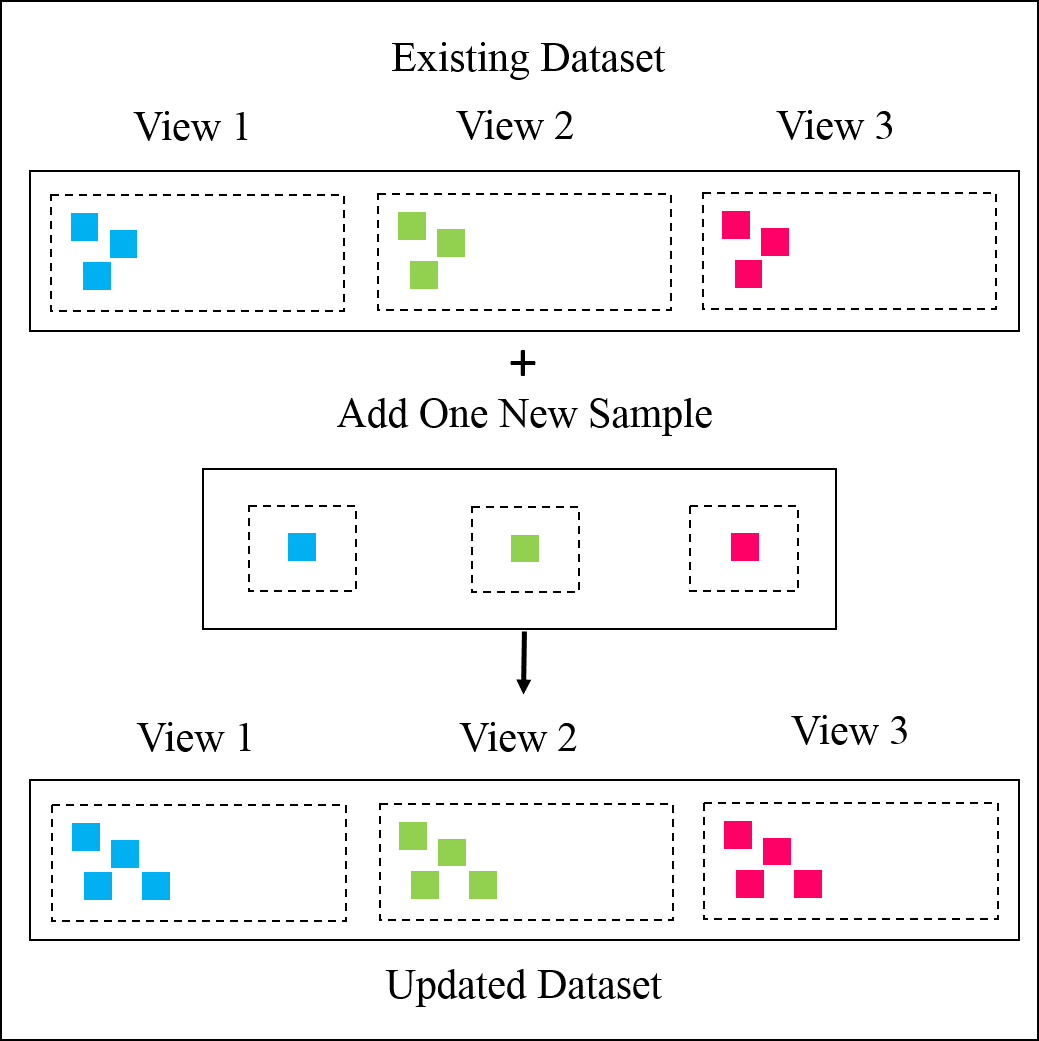
\includegraphics[width=\textwidth]{Figures/MvIDA/Fig1a.png}
		\caption{Sequential Increment and Existing Class}
		\label{fig:MvIDA_Intro_SeqEx}
	\end{subfigure}\hspace{0.8cm}
	\begin{subfigure}[t]{0.45\textwidth}
		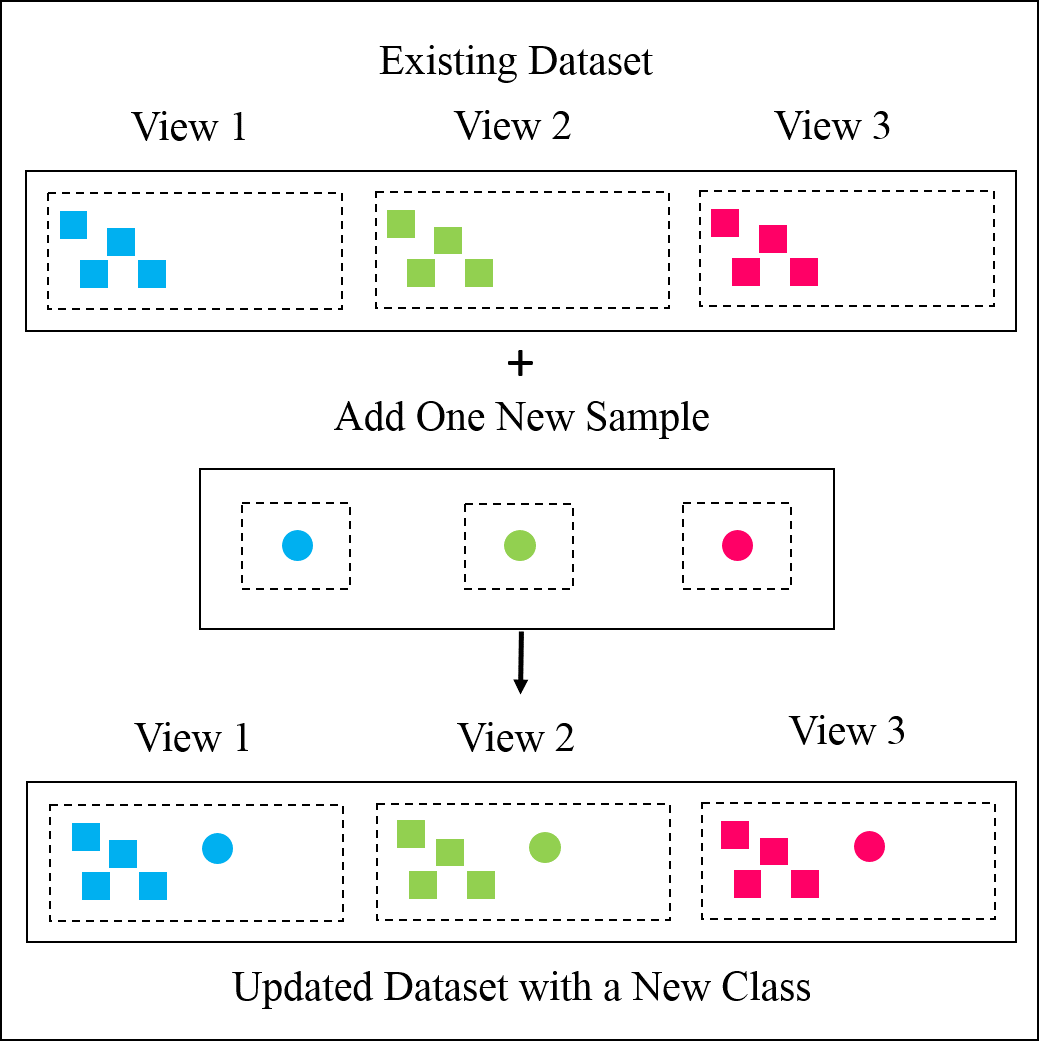
\includegraphics[width=\textwidth]{Figures/MvIDA/Fig1b.png}
		\caption{Sequential Increment and New Class}
		\label{fig:MvIDA_Intro_SeqNew}
	\end{subfigure}
	
\vspace{0.5cm}

	\begin{subfigure}[t]{0.45\textwidth}
		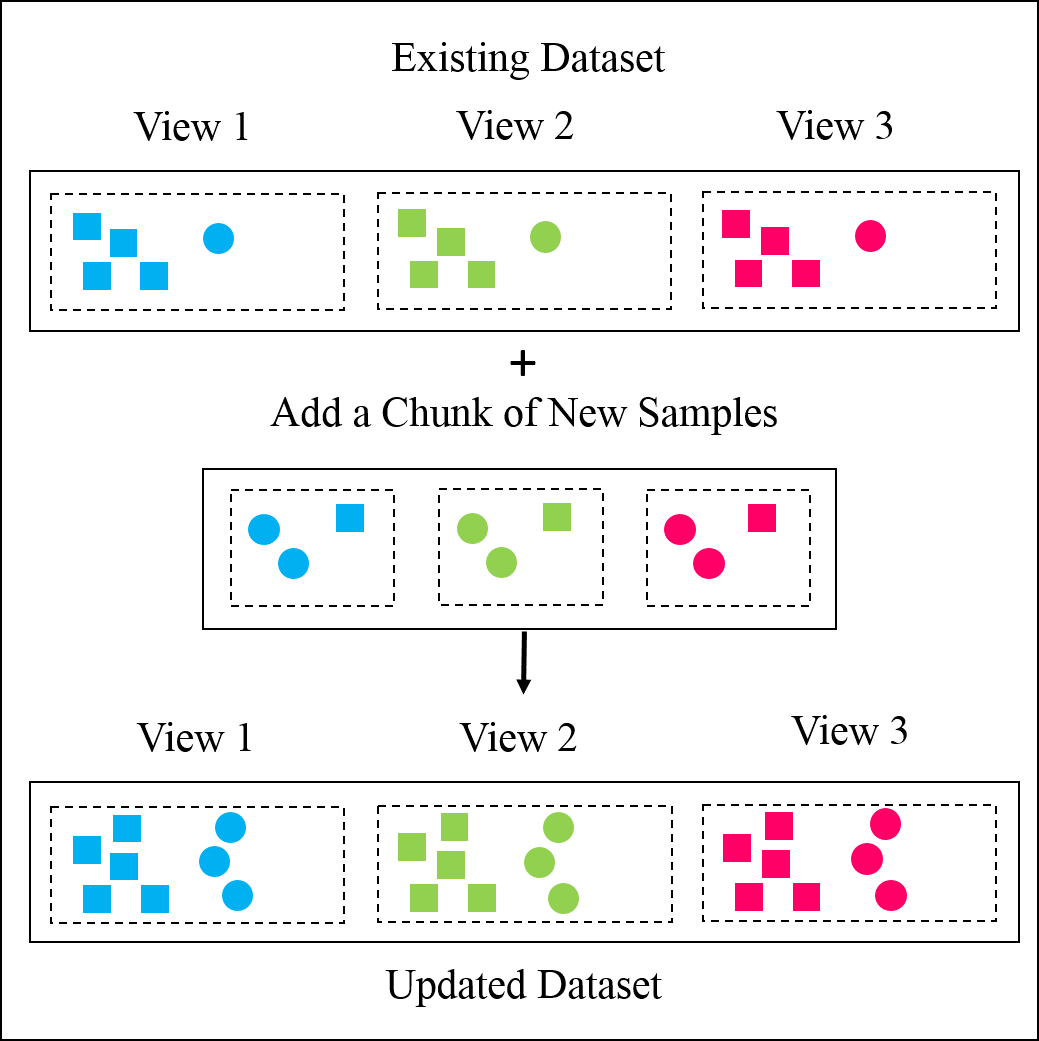
\includegraphics[width=\textwidth]{Figures/MvIDA/Fig2a.png}
		\caption{Chunk Increment and Existing Class}
		\label{fig:MvIDA_Intro_ChkEx}
	\end{subfigure}\hspace{0.8cm}
	\begin{subfigure}[t]{0.45\textwidth}
		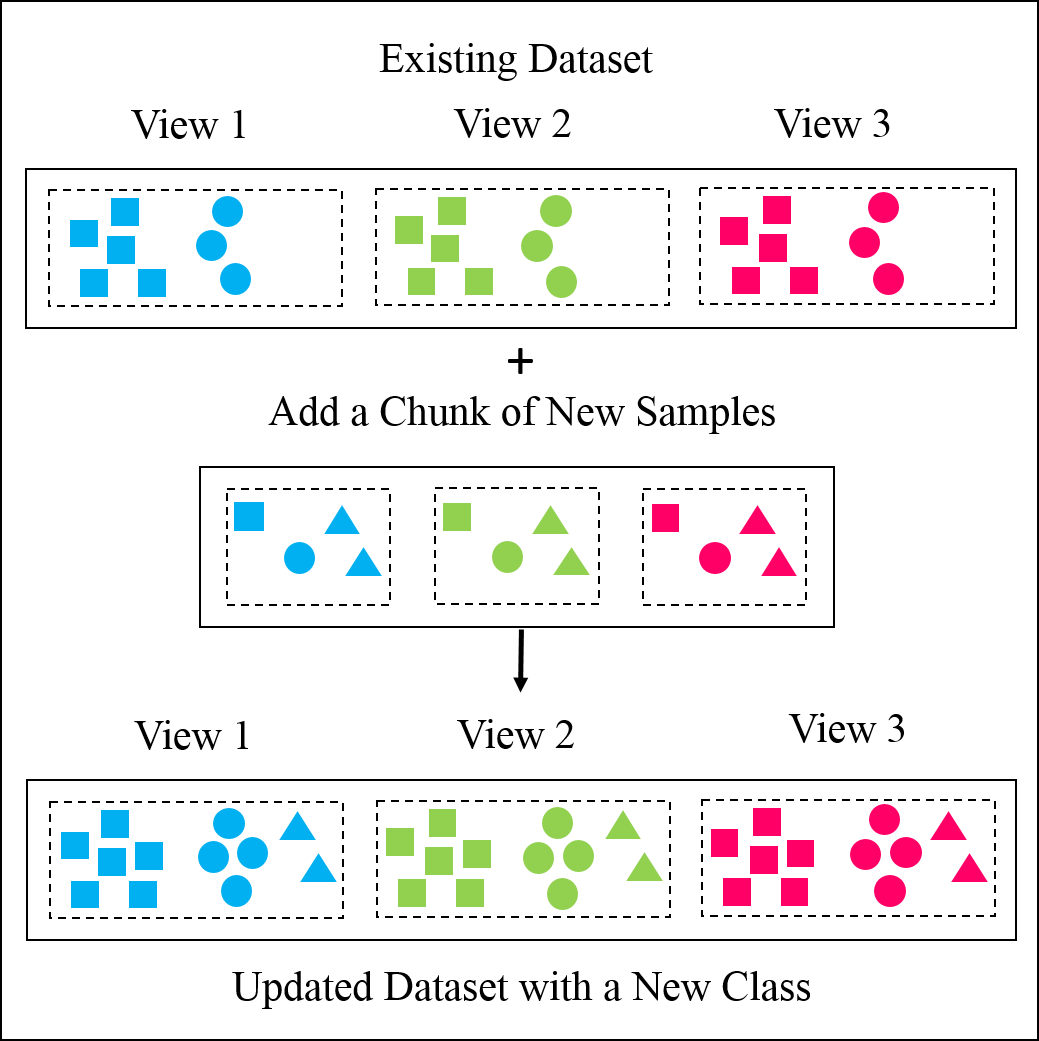
\includegraphics[width=\textwidth]{Figures/MvIDA/Fig2b.png}
		\caption{Chunk Increment and New Class}
		\label{fig:MvIDA_Intro_ChkNew}
	\end{subfigure}
	\caption{Cases of Increment: (a) A new data sample is added to every view. It belongs to an existing class. (b) A new data sample is added to every view. It belongs to a new class. (c) A chunk of new data samples is added. None of the new data samples belong to a new class. (d) A chunk of new data samples is added. Some of the new data samples belong to a new class.}
	\label{fig:MvIDA_Intro}
\end{figure}

We first present the methodology of MvIDA, and then the experimental setup and results are presented. We have compared MvIDA with its batch multi-view counterpart MvDA and single-view incremental counterpart Incremental Linear Discriminant Analysis (ILDA). We conclude this chapter by summarizing the features of the proposed method.










\section{Methodology}
\label{sec:MvIDA_Algo}
MvIDA has four different cases depending on the nature of an incoming data stream and the class labels of new data samples.
\begin{itemize}
	\item \textbf{Sequential increment and Existing class}- To be used when only one new sample is added at a time and it belongs to one of the already existing classes (Refer fig. \ref{fig:MvIDA_Intro_SeqEx}).
	\item \textbf{Sequential increment and New class}- To be used when only one new sample is added at a time and it belongs to a new class (Refer fig. \ref{fig:MvIDA_Intro_SeqNew}).

	\clearpage

	\item \textbf{Chunk increment and Existing class}- To be used when a group of new samples is added at a time and none of the new samples belongs to a new class (Refer fig. \ref{fig:MvIDA_Intro_ChkEx}).
	\item \textbf{Chunk increment and New class}- To be used when a group of new samples is added at a time and some of the new samples belong to new classes (Refer fig. \ref{fig:MvIDA_Intro_ChkNew}).
\end{itemize}

Each of the four cases of MvIDA follows four steps that incrementally update- (i) number of data samples, (ii) means, (iii) within-class scatter matrix, and (iv) between-class scatter matrix, respectively. Once these entities are updated, the new scatter matrices are used to find optimal projection vectors using Eq.(\ref{eqn:Lit_MvDA_GEP}). Algorithm \ref{MvIDA_Algo} presents the workings of MvIDA.





\subsection{Sequential Increment and Existing Class}
\label{subs:MvIDA_SeqEC}
Let us suppose only one data sample is added to the base set at a time and it belongs to an already existing class $E$. Let us denote this data sample by 
$\bar{\mathcal{X}} = \{ \bar{\textbf{x}}_{j} | j=1,\cdots,v \} $ and $\bar{\textbf{x}}_j \in \mathbb{R}^{p_j}$. Let $\bar{\mathcal{Y}} = \{ \bar{\textbf{y}}_{j} = \textbf{W}_j^T \bar{\textbf{x}}_{j} | j=1,\cdots,v \} $ be the projection of $\bar{\mathcal{X}}$ onto the common discriminant space.

\subsubsection{Updating the number of data samples}
\label{ssubs:MvIDA_SeqEC_n}
As the class already exists in $\mathcal{C}$, we have to update the number of total data samples ($n$), the number of data samples in class $E$ ($n_{E}$), and the number of data samples per class per view of class $E$ ($n_{Ej}$). The means $n_{ij}$ and $n_i$ for other classes $i \in \mathcal{C}-\{E\}$ do not change.

\begin{center}
$n'_{Ej} = n_{Ej}+1, \hspace{0.2cm} n'_E = n_E+v$ and $\hspace{0.2cm} n' = n+v$
\end{center}



\subsubsection{Updating the means}
\label{ssubs:MvIDA_SeqEC_mu}
As the new data sample has been added to class $E$, we update the means per class per view (${\textbf{m}_{Ej}}^{(x)}$) and class mean ($\textbf{m}_{E}$) of class $E$. The means of remaining classes do not need updating as these classes were not updated in the increment. We also update the total mean ($\textbf{m}$).

\begin{equation}
\label{eqn:1muij}
{\textbf{m}_{Ej}'}^{(x)} = \frac{ n_{Ej} {\textbf{m}_{Ej}}^{(x)} + \bar{\textbf{x}}_{j}}{n_{Ej}+1}
\end{equation}
\begin{equation}
\label{eqn:1mui}
\textbf{m}'_{E} = \frac{n_E \textbf{m}_{E} + v\bar{\textbf{m}}_{E}}{n_E + v} = \frac{n_E \textbf{m}_{E} + \sum_{j=1}^{v} \bar{\textbf{y}}_{j}}{n_E + v}
\end{equation}
\begin{equation}
\label{eqn:1mu}
\textbf{m}' = \frac{n \textbf{m} + v \bar{\textbf{m}}}{n+v} = \frac{n \textbf{m} + \sum_{j=1}^{v} \bar{\textbf{y}}_{j}}{n+v}  
\end{equation}



\subsubsection{Updating the within-class scatter matrix}
\label{ssubs:MvIDA_SeqEC_Sw}
As the within-class scatter of classes other than $E$ does not change, we only update the scatter of class $E$. The scatter of the rest of the classes does not need recomputing.

\vspace{-0.3cm}
\begin{equation}
\label{eqn:1Sw}
\begin{split}
\textbf{S}_W' = & \sum_{i=1,i \neq E}^{c} {\textbf{S}_{W_i}} + {\textbf{S}_{W_E}'} \\
= & \; \textbf{S}_W + \frac{v \; n_E}{(n_E+v)} \left ( \bar{\textbf{m}}_E - \textbf{m}_E \right ) \left ( \bar{\textbf{m}}_E - \textbf{m}_E \right )^T + \sum_{j=1}^{v} \left ( \bar{\textbf{y}_{j}} - \textbf{m}_E \right ) \left ( \bar{\textbf{y}_{j}} - \textbf{m}_E \right )^T
\end{split}
\end{equation}

\clearpage


\begin{algorithm}[t]
\centering
\caption{MvIDA algorithm}
\label{MvIDA_Algo}
    \begin{algorithmic}
	\STATE \textbf{Input :}
	\STATE - A trained model $\phi$ that consists of:
	\STATE 		\hspace{0.3cm} - Data sample counts: $n$, $n_i$, $n_{ij}$
	\STATE 		\hspace{0.3cm} - Means: $\textbf{m}$, $\textbf{m}_i$, $\textbf{m}_{ij}$
	\STATE 		\hspace{0.3cm} - Scatter matrices: $\textbf{S}$, $\textbf{D}$
	\STATE 		\hspace{0.3cm} - Set of class labels of existing data samples: $\mathcal{C}$
	\STATE 		- Set of new data samples: $\bar{\mathcal{X}}$
	\STATE 		- Number of new data samples: $\bar{n}$
	\STATE 		- Set of class labels of new data samples: $\bar{\mathcal{C}}$ \vspace{0.1cm}

	\WHILE{new data is encountered}
		\IF{$\bar{n}==1$}
		
			\IF{$\bar{\mathcal{C}} \in \mathcal{C}$}
				\STATE \small Update $n$, $n_i$, $n_{ij}$\;
				\STATE \small Update $\textbf{m}$, $\textbf{m}_i$, $\textbf{m}_{ij}$ using Eq.(\ref{eqn:1muij})-(\ref{eqn:1mu})\;
				\STATE \small Update $\textbf{S}$ using Eq.(\ref{eqn:1Sjr})\;
				\STATE \small Update $\textbf{D}$ using Eq.(\ref{eqn:1Djr})\;
			\ELSE
				\STATE \small Update $n$, $n_i$, $n_{ij}$\;
				\STATE \small Update $\textbf{m}$, $\textbf{m}_i$, $\textbf{m}_{ij}$ using Eq.(\ref{eqn:2muij})-(\ref{eqn:2mu})\;
				\STATE \small Update $\textbf{S}$ using Eq.(\ref{eqn:2Sjr})\;
				\STATE \small Update $\textbf{D}$ using Eq.(\ref{eqn:2Djr})\;
				\STATE $\mathcal{C} = \mathcal{C} \cup \bar{\mathcal{C}}$
			\ENDIF

		\ELSE
		
			\IF{$\bar{\mathcal{C}} \in \mathcal{C}$}
				\STATE \small Update $n$, $n_i$, $n_{ij}$\;
				\STATE \small Update $\textbf{m}$, $\textbf{m}_i$, $\textbf{m}_{ij}$ using Eq.(\ref{eqn:3muij})-(\ref{eqn:3mu})\;
				\STATE \small Update $\textbf{S}$ using Eq.(\ref{eqn:3Sjr})\;
				\STATE \small Update $\textbf{D}$ using Eq.(\ref{eqn:3Djr})\;

			\ELSE

				\STATE \small Update $n$, $n_i$, $n_{ij}$\;
				\STATE \small Update $\textbf{m}$, $\textbf{m}_i$, $\textbf{m}_{ij}$ using Eq.(\ref{eqn:4muij})-(\ref{eqn:4mu})\;
				\STATE \small Update $\textbf{S}$ using Eq.(\ref{eqn:4Sjr})\;
				\STATE \small Update $\textbf{D}$ using Eq.(\ref{eqn:4Djr})\;
				\STATE $\mathcal{C} = \mathcal{C} \cup \bar{\mathcal{C}}$
			\ENDIF
			
		\ENDIF

		\STATE \small Compute the projection matrix $\textbf{W}^{opt}$ using Eq.(\ref{eqn:Lit_MvDA_GEP})\;
	\ENDWHILE
	\STATE \textbf{Output :}
	\STATE - Updated model $\phi$
	\STATE - The projection matrix $\textbf{W}^{opt}$

\end{algorithmic}
\end{algorithm}

\clearpage

\noindent
and the reformulation of above equation is,

\begin{equation}
\label{eqn:1Sjr}
\textbf{S}_{jr}' = \left\{\begin{matrix*}[l]
\textbf{S}_{jr} + \frac{n_E}{v (n_E+v)} \left ( \bar{\textbf{x}}_j - {\textbf{m}_{Ej}}^{(x)} \right ) \left ( \bar{\textbf{x}}_j - {\textbf{m}_{Ej}}^{(x)} \right )^T + \bar{\textbf{x}}_j {\bar{\textbf{x}}_j}^T - \frac{1}{v} \bar{\textbf{x}}_j {\bar{\textbf{x}}_j}^T & j=r \\[0.3cm] 
\textbf{S}_{jr} + \frac{n_E}{v (n_E+v)} \left ( \bar{\textbf{x}}_j - {\textbf{m}_{Ej}}^{(x)} \right ) \left ( \bar{\textbf{x}}_r - {\textbf{m}_{Er}}^{(x)} \right )^T - \frac{1}{v} \bar{\textbf{x}}_j {\bar{\textbf{x}}_r}^T & j \neq r
\end{matrix*}\right.
\end{equation}

\noindent
For detailed derivation of $\textbf{S}_{W}'$ and $\textbf{S}_{jr}'$ refer to Appendix-B.%\ref{proof:MvIDA_SeqEx}.




\subsubsection{Updating the between-class scatter matrix}
\label{ssubs:MvIDA_SeqEC_Sb}
The between-class scatter depends on the total mean and class means. Hence, it has to be recalculated as the total mean and the class mean of class $E$ are updated after the increment.


\begin{equation}
\begin{split}
\label{eqn:1Sb}
\textbf{S}_B' = \; & \sum_{i=1,i\neq E}^{c} n_{i} (\textbf{m}_{i} - \textbf{m}') (\textbf{m}_{i} - \textbf{m}')^T + n_{E}'(\textbf{m}_E' - \textbf{m}') (\textbf{m}_E' - \textbf{m}')^T\\
= \; & \sum_{i=1}^{c} n_{i}' (\textbf{m}_{i}' - \textbf{m}') (\textbf{m}_{i}' - \textbf{m}')^T
\end{split}
\end{equation}

\noindent
and the reformulated between-class scatter is,

\begin{equation}
\label{eqn:1Djr}
\begin{split}
\textbf{D}_{jr}' = \; \sum_{i=1}^{c} & \; \frac{n_{ij}' \; n_{ir}'}{n_{i}'} \; {\textbf{m}_{ij}'}^{(x)} {{\textbf{m}_{ir}'}^{(x)}}^T - \frac{1}{n'} \left (\sum_{i=1}^{c} n_{ij}' \; {\textbf{m}_{ij}'}^{(x)} \right ) \left (\sum_{i=1}^{c} n_{ir}' \; {{\textbf{m}_{ir}'}^{(x)}} \right )^T
\end{split}
\end{equation}

\noindent
For detailed derivation of $\textbf{S}_B'$ and $\textbf{D}_{jr}'$ refer to Appendix-A.%\ref{proof:Djr}.












\subsection{Sequential Increment and New Class}
\label{subs:MvIDA_SeqNC}
The second case is when the newly added data sample belongs to a new class $N$. Let us denote this data sample by 
$\bar{\mathcal{X}} = \{ \bar{\textbf{x}}_{j} | j=1,\cdots,v \} $ and $\bar{\textbf{x}}_j \in \mathbb{R}^{p_j}$. Let $\bar{\mathcal{Y}} = \{ \bar{\textbf{y}}_{j} = \textbf{W}_j^T \bar{\textbf{x}}_{j} | j=1,\cdots,v \} $ be the projection of $\bar{\mathcal{X}}$ onto the common discriminant space.


\subsubsection{Updating the number of data samples}
\label{ssubs:MvIDA_SeqNC_n}
As this is the first data sample in its class, we initialize the number of data samples per class per view for this new class as, $n_{Nj} = 1$. Also, the number of data samples per class, $n_N = v$ and updated total number of data samples, $n' = n + v$. Both, $n_{ij}$ and $n_i$ for $i \in \mathcal{C}$ do not change.



\subsubsection{Updating the means}
\label{ssubs:MvIDA_SeqNC_mu}
\begin{equation}
\label{eqn:2muij}
{\textbf{m}_{Nj}'}^{(x)} = {\bar{\textbf{m}}_{Nj}}^{(x)} = \bar{\textbf{x}}_{j}
\end{equation}
\begin{equation}
\label{eqn:2mui}
\textbf{m}_{N}' = \bar{\textbf{m}}_{N} = \frac{1}{v} \sum_{j=1}^{v} \textbf{y}_{j}'
\end{equation}
\begin{equation}
\label{eqn:2mu}
\textbf{m}' = \frac{n\textbf{m} + v \bar{\textbf{m}}}{n+v} = \frac{n\textbf{m} + \sum_{j=1}^{v} \bar{\textbf{y}_{j}}}{n+v}
\end{equation}



\subsubsection{Updating the within-class scatter matrix}
\label{ssubs:MvIDA_SeqNC_Sw}
We only add the within-class scatter of the new class to the old $\textbf{S}_W$, as the within-class scatter of existing classes does not change.

\begin{equation}
\label{eqn:2Sw}
\textbf{S}_W' = \textbf{S}_W+\sum_{j=1}^{v}(\bar{\textbf{y}}_j - \bar{\textbf{m}}_{N})(\bar{\textbf{y}}_j - \bar{\textbf{m}}_{N})^T
\end{equation}

\noindent
and the reformulation of above equation is, 

\begin{equation}
\label{eqn:2Sjr}
\begin{split}
\textbf{S}_{jr}' = \left\{\begin{matrix*}[l]
\textbf{S}_{jr} + \bar{\textbf{x}}_{j} \; {\bar{\textbf{x}}_{j}}^T - \frac{1}{v^2} \bar{\textbf{x}}_j \; {\bar{\textbf{x}}_j}^T & j=r \\[0.3cm]
\textbf{S}_{jr} - \frac{1}{v^2} \bar{\textbf{x}}_j \; {\bar{\textbf{x}}_r}^T & j \neq r
\end{matrix*}\right.
\end{split}
\end{equation}

\noindent
For detailed derivation of $\textbf{S}_{W}'$ and $\textbf{S}_{jr}'$ refer to Appendix-C.%\ref{proof:MvIDA_SeqNew}.



\subsubsection{Updating the between-class scatter matrix}
\label{ssubs:MvIDA_SeqNC_Sb}
Like before, the between-class scatter has to be recalculated as,

\begin{equation}
\label{eqn:2Sb}
\begin{split}
\textbf{S}_B' = \; & \sum_{i=1}^{c} n_{i} (\textbf{m}_{i} - \textbf{m}') (\textbf{m}_{i} - \textbf{m}')^T + v(\bar{\textbf{m}}_N - \textbf{m}') (\bar{\textbf{m}}_N - \textbf{m}')^T\\
= \; & \sum_{i=1}^{c+1} n_{i}' (\textbf{m}_{i}' - \textbf{m}') (\textbf{m}_{i}' - \textbf{m}')^T \end{split}
\end{equation}

\noindent
and the reformulated between-class scatter is,

\begin{equation}
\label{eqn:2Djr}
\begin{split}
\textbf{D}_{jr}' = \; \sum_{i=1}^{c+1} & \; \frac{n_{ij}' \; n_{ir}'}{n_{i}'} \; {\textbf{m}_{ij}'}^{(x)} {{\textbf{m}_{ir}'}^{(x)}}^T - \frac{1}{n'} \left (\sum_{i=1}^{c+1} n_{ij}' \; {\textbf{m}_{ij}'}^{(x)} \right ) \left (\sum_{i=1}^{c+1} n_{ir}' \; {{\textbf{m}_{ir}'}^{(x)}} \right )^T
\end{split}
\end{equation}

\noindent
After the completion of all four steps, we add the new class in the set of existing classes ($\mathcal{C}$).








\subsection{Chunk Increment and Existing Class}
\label{subs:MvIDA_ChkEC}
For the first case of chunk increment, $\bar{n}_i$ of the $\bar{n}$ new data samples belong to class $i \in \mathcal{C}$, meaning, none of the new data samples belong to a class that has not yet been introduced. We denote a chunk of new data samples by, $\bar{\mathcal{X}} = \{ \bar{\textbf{x}}_{ijk} | i=1,\cdots,c; j=1,\cdots,v; k=1,\cdots,\bar{n}_{ij} \}$ and $\bar{\textbf{x}}_{ijk} \in \mathbb{R}^{p_j}$. Let $\bar{\mathcal{Y}} = \{ \bar{\textbf{y}}_{ijk} = \textbf{W}_j^T \bar{\textbf{x}}_{ijk} | i=1,\cdots,c; j=1,\cdots,v; k=1,\cdots,\bar{n}_{ij} \}$ be the projection of $\bar{\mathcal{X}}$ onto the common discriminant space.



\subsubsection{Updating the number of data samples}
\label{ssubs:MvIDA_ChkEC_n}
\begin{center}
$n'_{ij} = n_{ij} + \bar{n}_{ij}, \hspace{0.2cm} n'_i = n_i + \bar{n}_i$ and $\hspace{0.2cm} n' = n + \bar{n}$
\end{center}
for $i=1,\cdots,c$ and $j=1,\cdots,v$.



\subsubsection{Updating the means}
\label{ssubs:MvIDA_ChkEC_mu}
\begin{equation}
\label{eqn:3muij}
{\textbf{m}_{ij}'}^{(x)} = \frac{ n_{ij} {\textbf{m}_{ij}}^{(x)} + \bar{n}_{ij} \bar{\textbf{m}_{ij}}^{(x)}} {n_{ij} + \bar{n}_{ij}} = \frac{n_{ij} {\textbf{m}_{ij}}^{(x)} + \sum_{k=1}^{\bar{n}_{ij}} \bar{\textbf{x}}_{ijk}}{n_{ij} + \bar{n}_{ij}}
\end{equation}
\begin{equation}
\label{eqn:3mui}
\textbf{m}'_{i} = \frac{n_i \textbf{m}_{i} + \bar{n}_i \bar{\textbf{m}_{i}}}{n_i + \bar{n}_i} = \frac{n_i \textbf{m}_{i} + \sum_{j=1}^{v} \sum_{k=1}^{\bar{n}_{ij}} \bar{\textbf{y}}_{ijk}}{n_i + \bar{n}_i}
\end{equation}
\begin{equation}
\label{eqn:3mu}
\textbf{m}' = \frac{n \textbf{m} + \bar{n} \bar{\textbf{m}}}{n+\bar{n}} = \frac{n \textbf{m} + \sum_{i=1}^{c} \sum_{j=1}^{v} \sum_{k=1}^{\bar{n}_{ij}} \bar{\textbf{y}}_{ijk}}{n+\bar{n}}
\end{equation}



\subsubsection{Updating the within-class scatter matrix}
\label{ssubs:MvIDA_ChkEC_Sw}
The within-class scatter of only the classes to which new data samples were added is updated. Hence, we have,

\begin{equation}
\label{eqn:3Sw}
\begin{split}
\textbf{S}_W' = \textbf{S}_W + \sum_{i=1}^{c} & \Bigg[ \sum_{j=1}^{v} \sum_{k=1}^{\bar{n}_{ij}} \left ( \bar{\textbf{y}}_{ijk} {\bar{\textbf{y}}_{ijk}}^T - \bar{\textbf{y}}_{ijk} {\textbf{m}_i}^T \right ) + \frac{\bar{n}_{i} n_{i}}{(n_{i}+\bar{n}_{i})} \left ( \bar{\textbf{m}}_i - \textbf{m}_{i} \right ) \left ( \bar{\textbf{m}}_i - \textbf{m}_{i} \right )^T  \Bigg]
\end{split}
\end{equation}

\noindent
and the reformulation of above equation is, 

\begin{equation}
\label{eqn:3Sjr}
\begin{split}
\textbf{S}_{jr}' = \left\{\begin{matrix*}[l]
\textbf{S}_{jj} + \sum\limits_{i=1}^{c} \bigg[ \frac{v \bar{n}_i + n_i}{\bar{n}_i n_i (n_i + \bar{n}_i)^2} \textbf{a} \textbf{a}^T - \frac{\bar{n}_{ij} \bar{n}_{ij}}{\bar{n}_i} \textbf{m}_{ij}^{(x)} \textbf{m}_{ij}^{(x)^T} + \sum\limits_{k=1}^{\bar{n}_{ij}} \bar{\textbf{x}}_{ijk} {\bar{\textbf{x}}_{ijk}}^T \bigg] & j=r \\[0.4cm]
\textbf{S}_{jr} + \sum\limits_{i=1}^{c} \bigg[ \frac{v \bar{n}_i + n_i}{\bar{n}_i n_i (n_i + \bar{n}_i)^2} \textbf{a} \textbf{b}^T - \frac{\bar{n}_{ij} \bar{n}_{ir}}{\bar{n}_i} \textbf{m}_{ij}^{(x)} \textbf{m}_{ir}^{(x)^T} \bigg] & j \neq r
\end{matrix*}\right.
\end{split}
\end{equation}

\noindent
Where,\\
$\textbf{a} = \bar{n}_{ij} n_i \bar{\textbf{m}}_{ij}^{(x)} - \bar{n}_i n_{ij} \textbf{m}_{ij}^{(x)}$ and $\textbf{b} = \bar{n}_{ir} n_i \bar{\textbf{m}}_{ir}^{(x)} - \bar{n}_i n_{ir} \textbf{m}_{ir}^{(x)}$

\noindent
For detailed derivation of $\textbf{S}_{W}'$ and $\textbf{S}_{jr}'$ refer to Appendix-D.%\ref{proof:MvIDA_ChunkEx}.



\subsubsection{Updating the between-class scatter matrix}
\label{ssubs:MvIDA_ChkEC_Sb}
The between-class scatter is recalculated as,

\begin{equation}
\label{eqn:3Sb}
\textbf{S}_B' = \sum_{i=1}^{c} n_{i}' (\textbf{m}_{i}' - \textbf{m}') (\textbf{m}_{i}' - \textbf{m}')^T
\end{equation}

\noindent
and the reformulated between-class scatter is,

\begin{equation}
\label{eqn:3Djr}
\begin{split}
\textbf{D}_{jr}' = \; \sum_{i=1}^{c} & \; \frac{n_{ij}' \; n_{ir}'}{n_{i}'} \; {\textbf{m}_{ij}'}^{(x)} {{\textbf{m}_{ir}'}^{(x)}}^T - \frac{1}{n'} \left (\sum_{i=1}^{c} n_{ij}' \; {\textbf{m}_{ij}'}^{(x)} \right ) \left (\sum_{i=1}^{c} n_{ir}' \; {{\textbf{m}_{ir}'}^{(x)}} \right )^T
\end{split}
\end{equation}





\subsection{Chunk Increment and New Class}
\label{subs:MvIDA_ChkNC}
In second case of chunk increment, we assume that out of $\bar{n}$ new data samples, some samples belong to new classes. The number of new classes may be one or more. Here, we denote a chunk of new data samples by, $\bar{\mathcal{X}} = \{ \bar{\textbf{x}}_{ijk} | i=1,\cdots,c'; j=1,\cdots,v; k=1,\cdots,\bar{n}_{ij} \}$ and $\bar{\textbf{x}}_{ijk} \in \mathbb{R}^{p_j}$. Here, $c'$ is the number of classes after adding the new classes. Let $\bar{\mathcal{Y}} = \{ \bar{\textbf{y}}_{ijk} = \textbf{W}_j^T \bar{\textbf{x}}_{ijk} | i=1,\cdots,c'; j=1,\cdots,v; k=1,\cdots,\bar{n}_{ij} \}$ be the projection of $\bar{\mathcal{X}}$ onto the common discriminant space.



\subsubsection{Updating the number of data samples}
\label{ssubs:MvIDA_ChkNC_n}
\begin{center}
$n'_{ij} = n_{ij} + \bar{n}_{ij}, \hspace{0.2cm} n'_i = n_i + \bar{n}_i$ and $\hspace{0.2cm} n' = n + \bar{n}$
\end{center}
for $i=1,\cdots,c'$ and $j=1,\cdots,v$.



\subsubsection{Updating the means}
\label{ssubs:MvIDA_ChkNC_mu}
\begin{equation}
\label{eqn:4muij}
{\textbf{m}_{ij}'}^{(x)} = \frac{ n_{ij} {\textbf{m}_{ij}}^{(x)} + \bar{n}_{ij} \bar{\textbf{m}_{ij}}^{(x)}} {n_{ij} + \bar{n}_{ij}} = \frac{n_{ij} {\textbf{m}_{ij}}^{(x)} + \sum_{k=1}^{\bar{n}_{ij}} \bar{\textbf{x}}_{ijk}}{n_{ij} + \bar{n}_{ij}}
\end{equation}
\begin{equation}
\label{eqn:4mui}
\textbf{m}'_{i} = \frac{n_i \textbf{m}_{i} + \bar{n}_i \bar{\textbf{m}}_{i}}{n_i + \bar{n}_i} = \frac{n_i \textbf{m}_{i} + \sum_{j=1}^{v} \sum_{k=1}^{\bar{n}_{ij}} \bar{\textbf{y}}_{ijk}}{n_i + \bar{n}_i}
\end{equation}
\begin{equation}
\label{eqn:4mu}
\textbf{m}' = \frac{n \textbf{m} + \bar{n} \bar{\textbf{m}}}{n+\bar{n}} = \frac{n \textbf{m} + \sum_{i=1}^{c} \sum_{j=1}^{v} \sum_{k=1}^{\bar{n}_{ij}} \bar{\textbf{y}}_{ijk}}{n+\bar{n}}
\end{equation}



\subsubsection{Updating the within-class scatter matrix}
\label{ssubs:MvIDA_ChkNC_Sw}
The within-class scatter of the existing and the new classes to which new data samples were added is updated. Hence, we have,

\begin{equation}
\label{eqn:4Sw}
\begin{split}
\textbf{S}_W' = \textbf{S}_W + \sum_{i=1}^{c'} & \Bigg[ \sum_{j=1}^{v} \sum_{k=1}^{\bar{n}_{ij}} \left ( \bar{\textbf{y}}_{ijk} {\bar{\textbf{y}}_{ijk}}^T - \bar{\textbf{y}}_{ijk} \bar{\textbf{m}_i}^T \right ) + \frac{\bar{n}_{i} n_{i}}{(n_{i}+\bar{n}_{i})} \left ( \bar{\textbf{m}}_i - \textbf{m}_{i} \right ) \left ( \bar{\textbf{m}}_i - \textbf{m}_{i} \right )^T  \Bigg]
\end{split}
\end{equation}

\noindent
and the reformulation of above equation is,

\begin{equation}
\label{eqn:4Sjr}
\begin{split}
\textbf{S}_{jr}' = \left\{\begin{matrix*}[l]
\textbf{S}_{jj} + \sum\limits_{i=1}^{c'} \bigg[ \frac{v \bar{n}_i + n_i}{\bar{n}_i n_i (n_i + \bar{n}_i)^2} \textbf{a} \textbf{a}^T - \frac{\bar{n}_{ij} \bar{n}_{ij}}{\bar{n}_i} \bar{\textbf{m}}_{ij}^{(x)} \bar{\textbf{m}}_{ij}^{(x)^T} + \sum\limits_{k=1}^{\bar{n}_{ij}} \bar{\textbf{x}}_{ijk} {\bar{\textbf{x}}_{ijk}}^T \bigg] & j=r \\[0.3cm]
\textbf{S}_{jr} + \sum\limits_{i=1}^{c'} \bigg[ \frac{v \bar{n}_i + n_i}{\bar{n}_i n_i (n_i + \bar{n}_i)^2} \textbf{a} \textbf{b}^T - \frac{\bar{n}_{ij} \bar{n}_{ir}}{\bar{n}_i} \bar{\textbf{m}}_{ij}^{(x)} \bar{\textbf{m}}_{ir}^{(x)^T} \bigg] & j \neq r
\end{matrix*}\right.
\end{split}
\end{equation}

\noindent
Where,\\
$\textbf{a} = \bar{n}_{ij} n_i \bar{\textbf{m}}_{ij}^{(x)} - \bar{n}_i n_{ij} \textbf{m}_{ij}^{(x)}$ and $\textbf{b} = \bar{n}_{ir} n_i \bar{\textbf{m}}_{ir}^{(x)} - \bar{n}_i n_{ir} \textbf{m}_{ir}^{(x)}$

\noindent
The derivation of $\textbf{S}_{W}'$ and $\textbf{S}_{jr}'$ in this case is the same as in Appendix-D%\ref{proof:MvIDA_ChunkEx}
, if we set $c=c'$. Hence, no separate derivation is included.



\subsubsection{Updating the between-class scatter matrix}
\label{ssubs:MvIDA_ChkNC_Sb}
The between-class scatter is recalculated as,

\begin{equation}
\label{eqn:4Sb}
\textbf{S}_B' = \sum_{i=1}^{c'} n_{i}' (\textbf{m}_{i}' - \textbf{m}') (\textbf{m}_{i}' - \textbf{m}')^T
\end{equation}

\noindent
and the reformulated between-class scatter is,

\begin{equation}
\label{eqn:4Djr}
\begin{split}
\textbf{D}_{jr}' = \; \sum_{i=1}^{c'} & \; \frac{n_{ij}' \; n_{ir}'}{n_{i}'} \; {\textbf{m}_{ij}'}^{(x)} {{\textbf{m}_{ir}'}^{(x)}}^T - \frac{1}{n'} \left (\sum_{i=1}^{c'} n_{ij}' \; {\textbf{m}_{ij}'}^{(x)} \right ) \left (\sum_{i=1}^{c'} n_{ir}' \; {{\textbf{m}_{ir}'}^{(x)}} \right )^T
\end{split}
\end{equation}

\noindent
After the completion of all four steps, we add the new classes in the set of existing classes ($\mathcal{C}$).

It is possible to obtain the formulations of \textit{chunk increment and existing class} if we set $c'=c$ in the formulations in Section \ref{subs:MvIDA_ChkNC}. We can also obtain the sequential increment formulations for both cases by setting $l=1$ in the two chunk increment formulations. As these formulations are inherently similar to the batch MvDA, we can derive the batch MvDA formulations from MvIDA formulations. This is based on the base requirement of incremental methods that the discriminant spaces obtained by the incremental method must be identical to that of the batch method.








\section{Experiments and Results}
\label{sec:MvIDA_Expt}

\subsection{Experimental Setup}
\label{subs:MvIDA_Expt_Setup}
We use three 1D datasets- Handwritten Digits, Caltech-7, and AwA- for our experiments. The datasets are divided randomly into two parts for the experiments. The first part contains 80\% of the total data samples and is used to simulate the increments for training. The second part is the test set that contains 20\% of the total data samples.

We train two separate models, $\phi_{A}$ and $\phi_{B}$, using MvIDA and batch MvDA method, respectively. For sequential increment, one training data sample is introduced at a time. At each increment, MvIDA updates $\phi_{A}$ to include the newly added sample using sequential increment formulations (refer Algorithm \ref{MvIDA_Algo}) and computes the new projection vectors. At the same time, batch MvDA discards $\phi_{B}$ to recompute the same on all of the $(n+1)$ samples together.

For chunk increment, MvIDA handles the fixed as well as varying chunk sizes. However, to demonstrate the effect of the chunk size, we perform four separate experiments by taking chunks of 50, 100, 150, and 200 data samples, respectively. Similar to the Sequential increment, MvIDA updates $\phi_{A}$ using chunk increment formulations (refer Algorithm \ref{MvIDA_Algo}) to include $\bar{n}$ new data samples in each increment. At the same time, batch MvDA recalculates $\phi_{B}$ altogether for all of the $(n+\bar{n})$ samples, where $\bar{n}$ is the chunk size. 

At the end of the training process we obtain the projection matrices, $\textbf{W}^{opt}_{A}$ and $\textbf{W}^{opt}_{B}$ from the final models $\phi_{A}$ and $\phi_{B}$ respectively. These projection matrices are used to project each test sample $\textbf{y}^{Test}$ onto the common discriminant subspace. We compute the distance of $\textbf{y}^{Test}$ from each class mean in the projected space as follows.

\begin{equation}
\label{eqn:EuDist}
d(\textbf{y}^{Test}, \textbf{m}_i) = \left \| \textbf{y}^{Test} - \textbf{m}_{i} \right \|_2
\end{equation}

for $i=1,2,\cdots,c$.

$\textbf{y}^{Test}$ is then assigned the label of the class to which it is found to be closest. i.e.,

\begin{equation}
label(\textbf{y}^{Test}) = \underset{i}{argmin} \;\; d(\textbf{y}^{Test}, \textbf{m}_i)
\end{equation}




\begin{figure}[t]
\centering
  \begin{subfigure}[h]{\textwidth}
    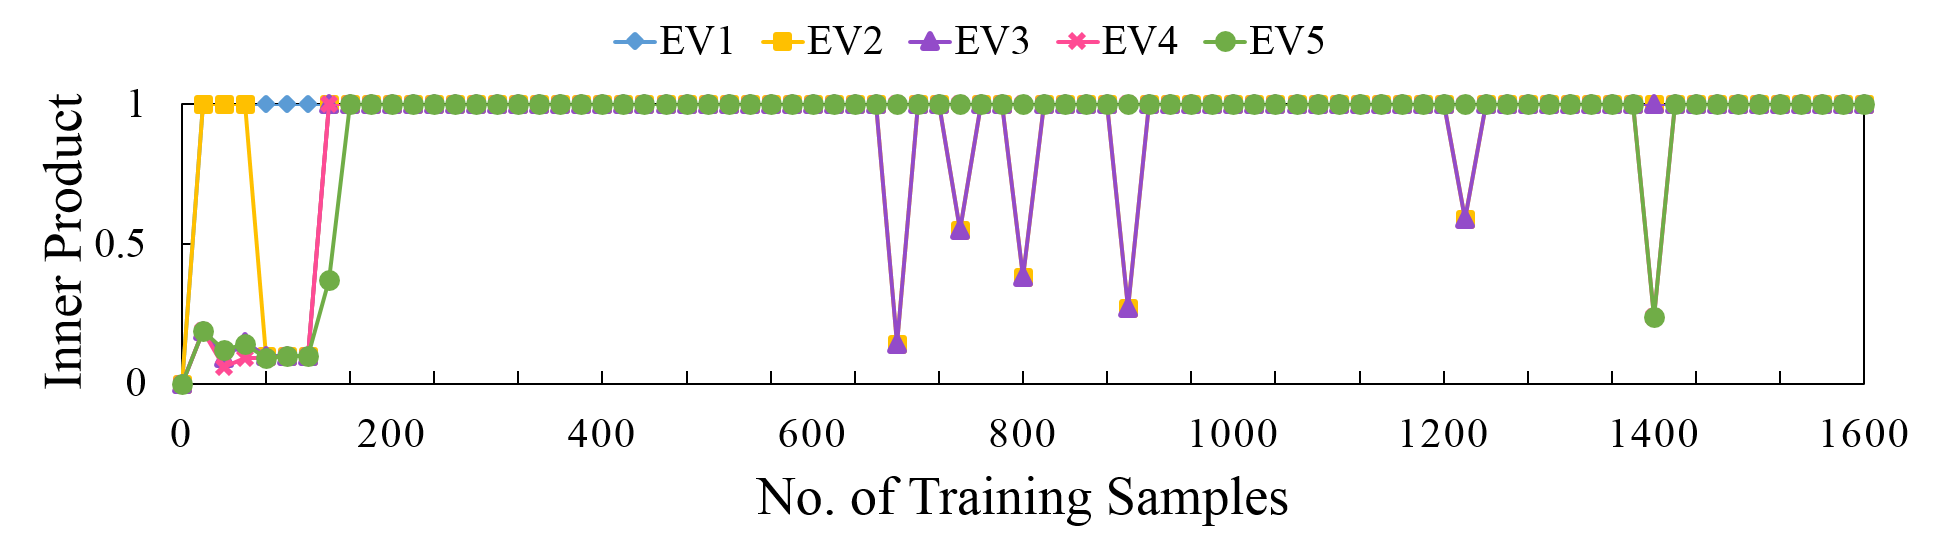
\includegraphics[width=0.95\textwidth]{Figures/MvIDA/Fig3.png}
    \caption{Handwritten digits dataset : Sequential increment}
  \end{subfigure}
  
  \begin{subfigure}[h]{\textwidth}
    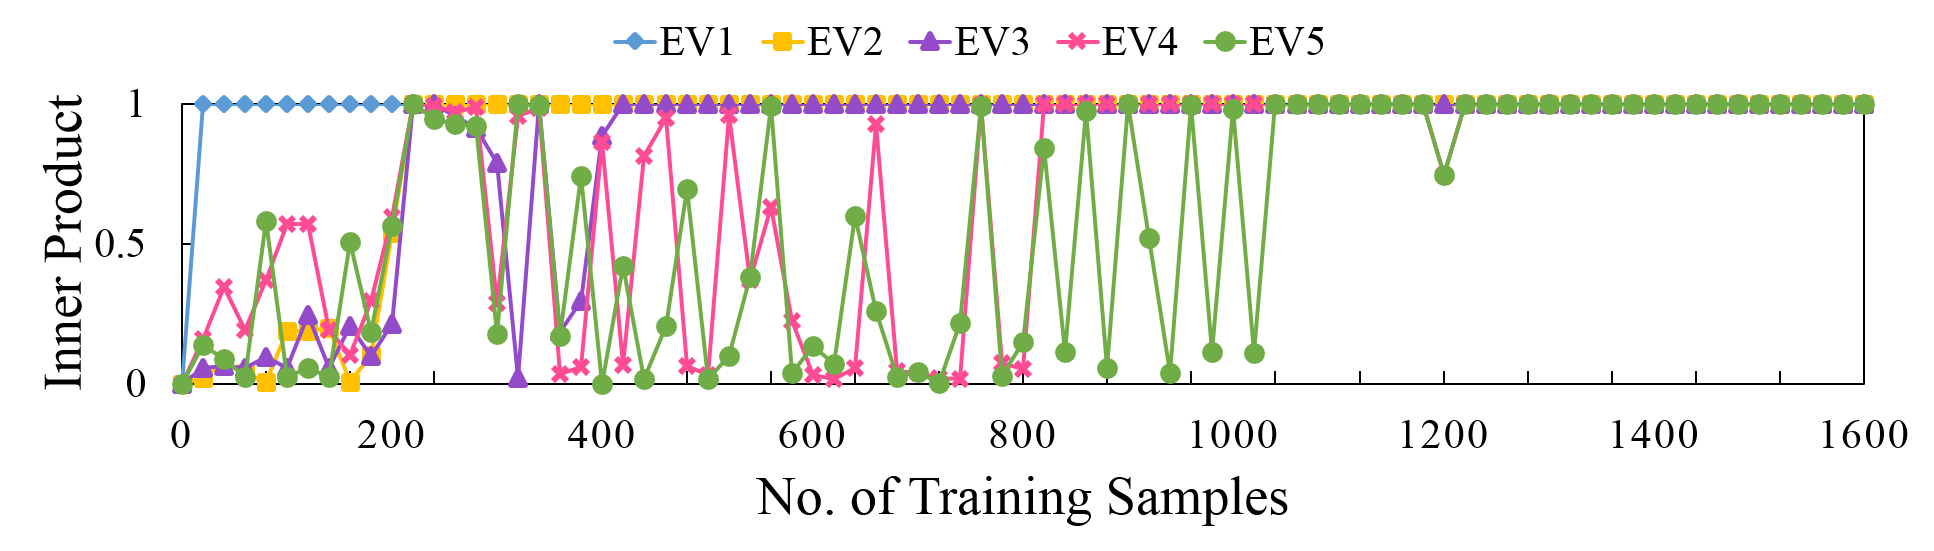
\includegraphics[width=0.95\textwidth]{Figures/MvIDA/Fig4.png}
    \caption{Handwritten digits dataset : Chunk increment}
  \end{subfigure}
\caption{Inner products of first five eigenvectors of MvIDA and batch MvDA for handwritten digits dataset.}
\label{fig:MvIDA_Eigs}
\end{figure}



\subsection{Results}
\label{subs:MvIDA_Res}
This section presents the results of experiments designed in order to answer the research questions posed in chapter \ref{ch:Intro}.

\subsubsection{Discriminative Subspace}
\label{ssubs:MvIDA_Subspace}

\begin{itemize}
\item \textbf{RQ1 :}
Can an incremental method, without using old data samples, produce an identical model to its batch counterpart MvDA?

\item \textbf{Experiment :}
We trained two models with MvIDA and batch MvDA, respectively. If the projection vectors obtained from both methods are in agreement with each other, the subspace, and in turn, the classification accuracy is also the same. Hence, we computed the inner product of the first five eigenvectors obtained from both methods. As the eigenvectors are of unit length, we say two eigenvectors are equal when their inner product is 1.

\item \textbf{Discussion :}
Fig.\ref{fig:MvIDA_Eigs} shows the inner product of the first five eigenvectors of batch MvDA and MvIDA computed on the Handwritten Digits dataset. The other two datasets also produce similar results and hence, are omitted. We see that the inner product of the first two eigenvectors of batch MvDA and MvIDA converges to 1 very early in both cases of increment. In the case of sequential increment, as only one data point is added at each increment, all of the eigenvectors converge faster with little to no changes. In the case of the chunk increment, a group of data samples is added in each increment. Hence, inner products of eigenvectors 3 to 5 see some fluctuations in the early stages of the progress before converging gradually to 1. This shows that the common discriminative subspace constructed by the proposed method evolves over the increments to achieve the same subspace as the batch method.

Fig. \ref{fig:MvIDA_Res_Vis} presents a t-SNE plot \cite{MaatenH08} of data samples in the projected space constructed by MvIDA and MvDA for handwritten digits dataset. Here, 0 to 9 are class labels that correspond to the digits from 0 to 9. We see that both the methods have formed the same projection space and hence have the same classification accuracy.
\end{itemize}


\begin{figure}[t]
\centering
  \begin{subfigure}[h]{0.65\textwidth}
    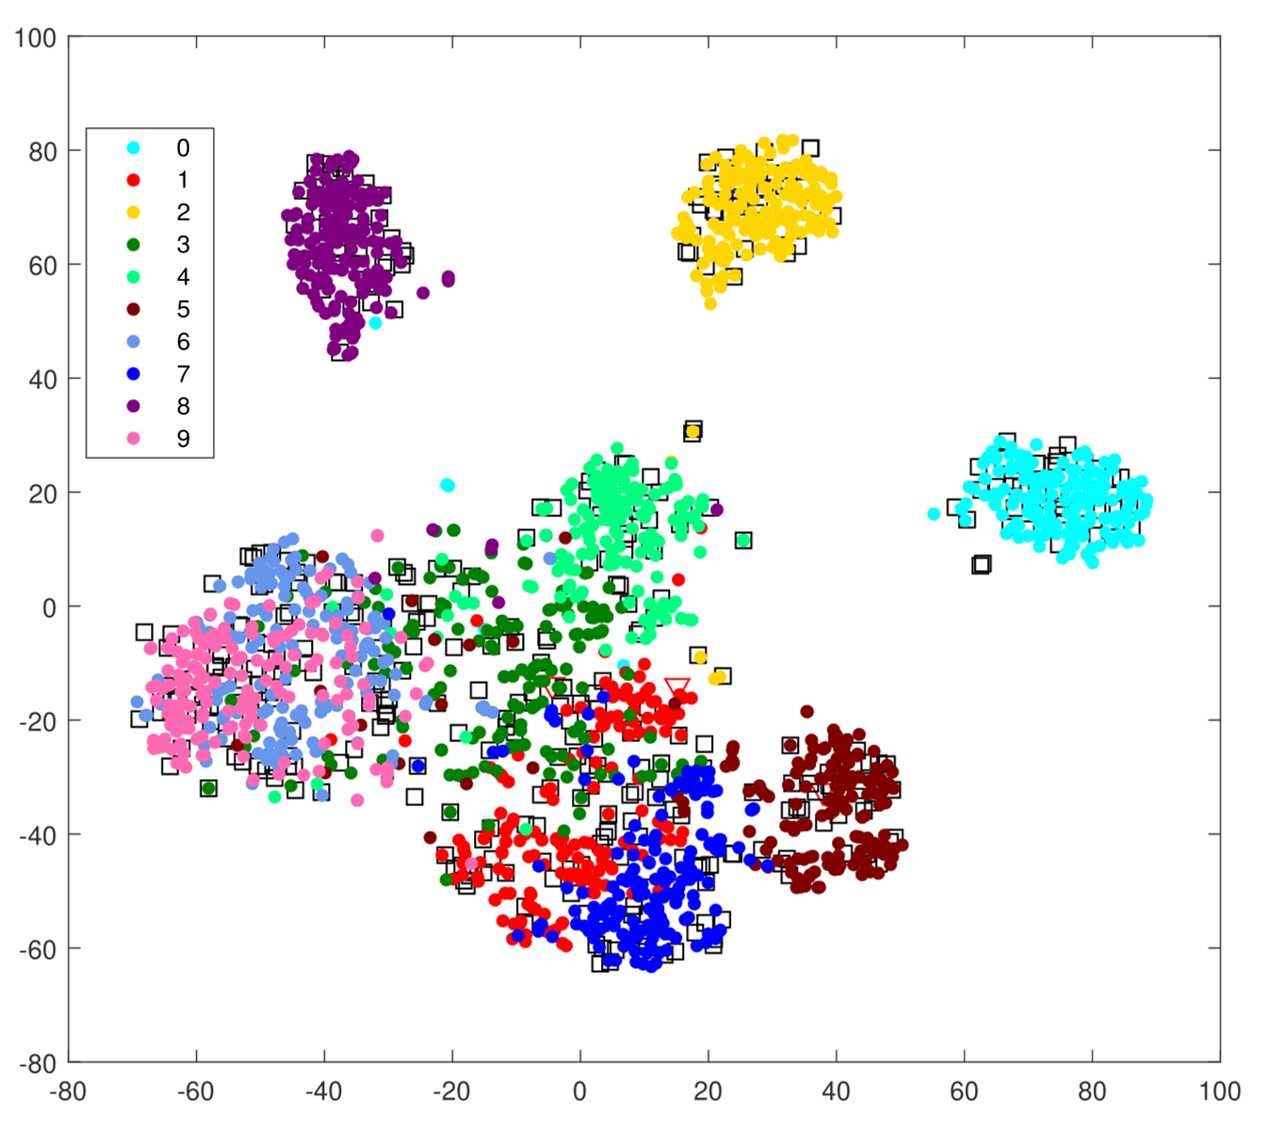
\includegraphics[width=\textwidth]{Figures/MvIDA/Fig5.png}
    \caption{{MvIDA}}
    \label{fig:MvIDA_Res_Vis_MvIDA}
  \end{subfigure}
  
  \begin{subfigure}[h]{0.65\textwidth}
    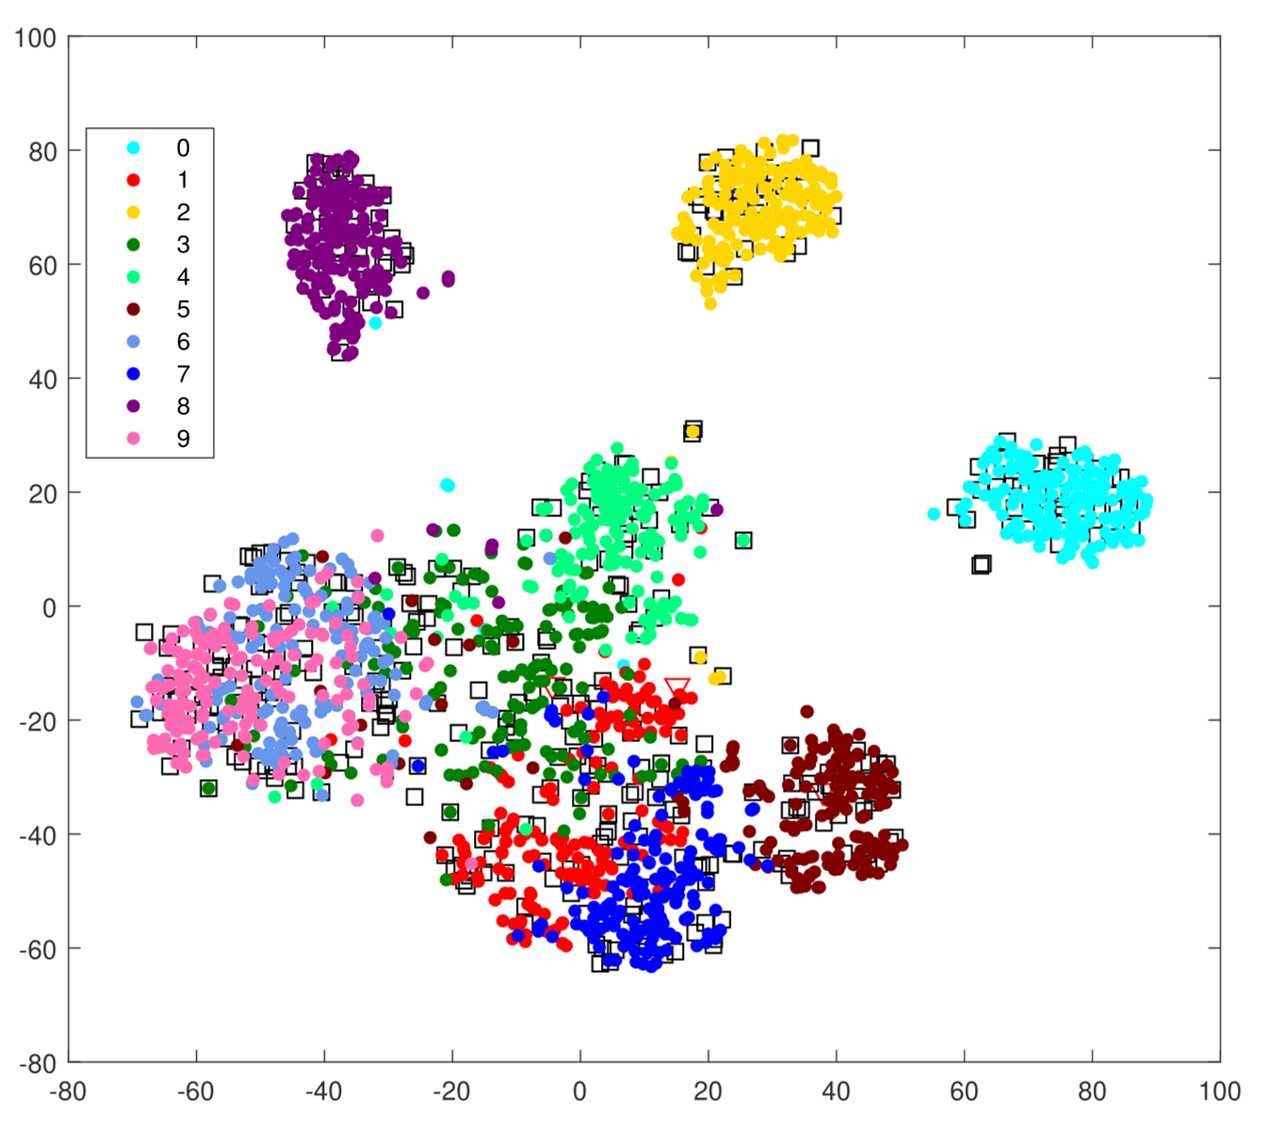
\includegraphics[width=\textwidth]{Figures/MvIDA/Fig6.png}
    \caption{{MvDA}}
    \label{fig:MvIDA_Res_Vis_MvDA}
  \end{subfigure}
\caption{A plot of data samples of the handwritten digits dataset in the projected space constructed by MvIDA and MvDA. Training data samples from different classes are shown in different colors. Correctly classified test samples are shown by black squares and incorrectly classified test samples are shown by red triangles.}
\label{fig:MvIDA_Res_Vis}
\end{figure}

\clearpage







\subsubsection{Order Independence}
\label{ssubs:MvIDA_OI}
\begin{itemize}
\item \textbf{RQ2 :}
Is this incremental method invariant to the order of addition of new data samples?

\item \textbf{Experiment :}
We performed 100 iterations of MvIDA by adding the data samples in randomized order every time. In the end, we compare the first five eigenvectors of all the iterations with that of batch MvDA.

\item \textbf{Discussion :}
Similar to the above experiment, the inner product of the projection vectors is 1 if the discriminant space constructed by all iterations is the same. We have included the results on the Handwritten Digits dataset here in Fig.\ref{fig:MvIDA_OI_DigChk}. Here, graphs of the eigenvectors overlap as all the values have converged to 1, proving the order independence of the proposed method.
\end{itemize}

\begin{figure}[t]
	\centering
	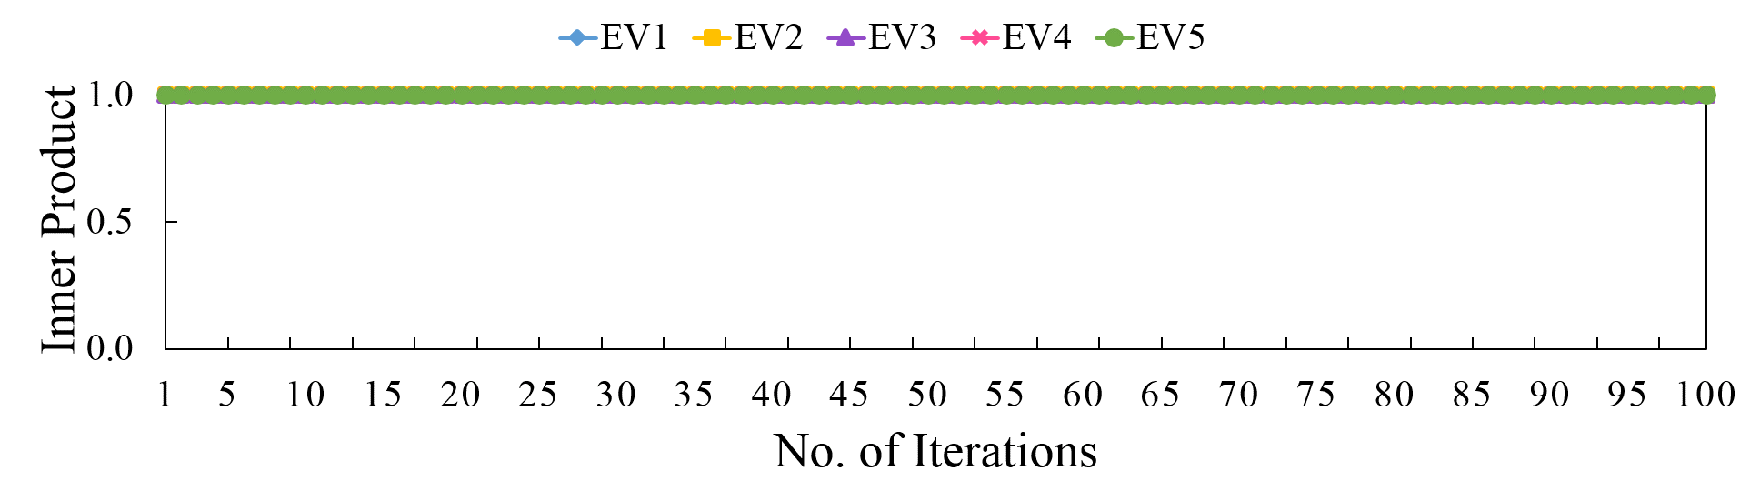
\includegraphics[width=\textwidth]{Figures/MvIDA/Fig7.pdf}
	\caption{Inner product of the first five eigenvectors of every iteration for handwritten digits dataset}
	\label{fig:MvIDA_OI_DigChk}
\end{figure}








\subsubsection{Training Time}
\label{ssubs:MvIDA_Time}
\begin{itemize}
\item \textbf{RQ3 :} 
Can this incremental method reduce training time?

\item \textbf{Experiment :}
We record the time taken by each method at the intervals of 50 data points for \textit{sequential} and \textit{chunk-50}. For \textit{chunk-100}, \textit{chunk-150} and \textit{chunk-200} the time is recorded at intervals of 100, 150 and 200 data samples respectively. Here, the time records for MvIDA consist of the time taken for updating the four entities, namely- the number of data sample, the means, the within-class scatter and the between-class scatter. Similarly, the time records for MvDA consist of the time taken for recomputing these four entities. We have not considered the time taken for the computation of the projection vectors, as this step is common for both the methods.

\item \textbf{Discussion :}
It is intuitive for MvIDA to require less time than batch MvDA, which is reflected in Fig. \ref{fig:MvIDA_Time_Seq}-\ref{fig:MvIDA_Time_Chk}. Note that for the AwA dataset, the unit of time is million seconds and the markers are placed sparsely for better viewing. Fig.\ref{fig:MvIDA_Time_Seq} shows the time comparison between MvIDA and batch MvDA for sequential increment on all four datasets. We see that MvIDA requires very less training time compared to batch MvDA. As the number of samples increases, the difference in the time grows larger. Sequential MvIDA took nearly 20 days to complete training on the AwA dataset. However, the batch MvDA is estimated to require around 912 days to complete the same. The dashed part of the Sequential MvDA curve in Fig.\ref{fig:MvIDA_Time_Seq_AwA} shows the estimated training time.




\begin{figure*}[t]
\centering
  \begin{subfigure}[h]{0.40\textwidth}
    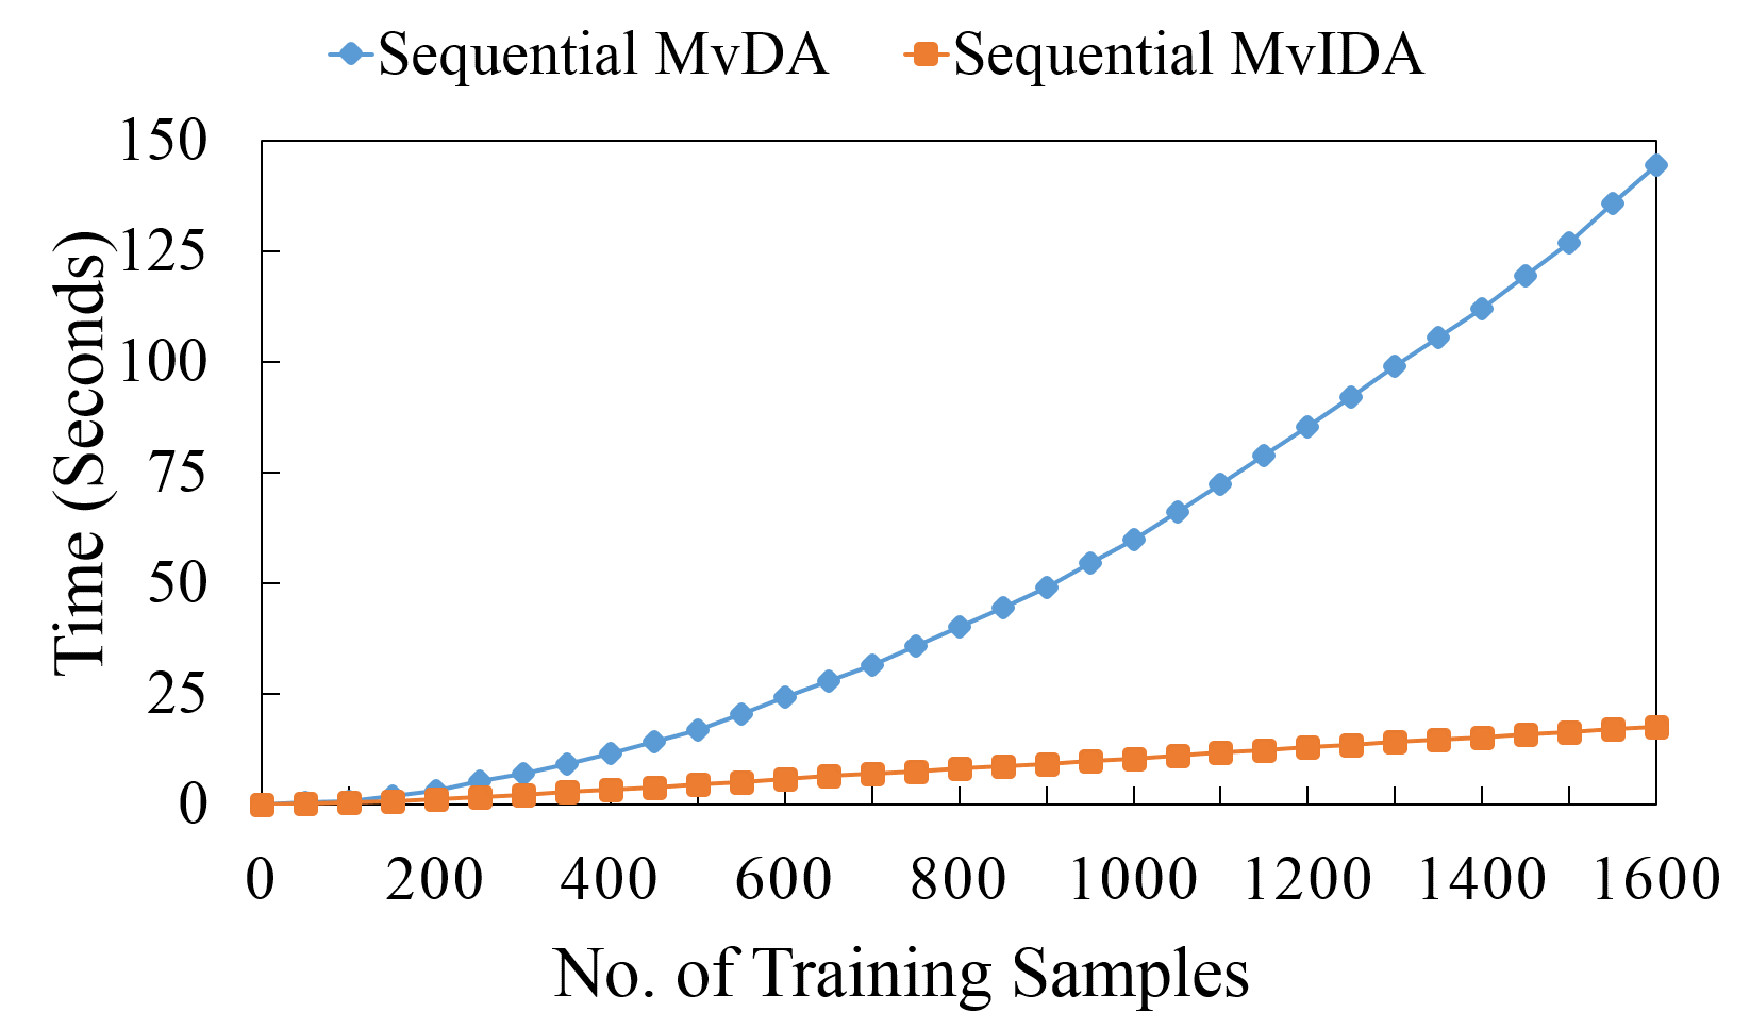
\includegraphics[width=\textwidth]{Figures/MvIDA/Fig8.pdf}
    \caption{{\scriptsize Handwritten Digits Dataset}}
    \label{fig:MvIDA_Time_Seq_Dig}
  \end{subfigure}
  \begin{subfigure}[h]{0.40\textwidth}
    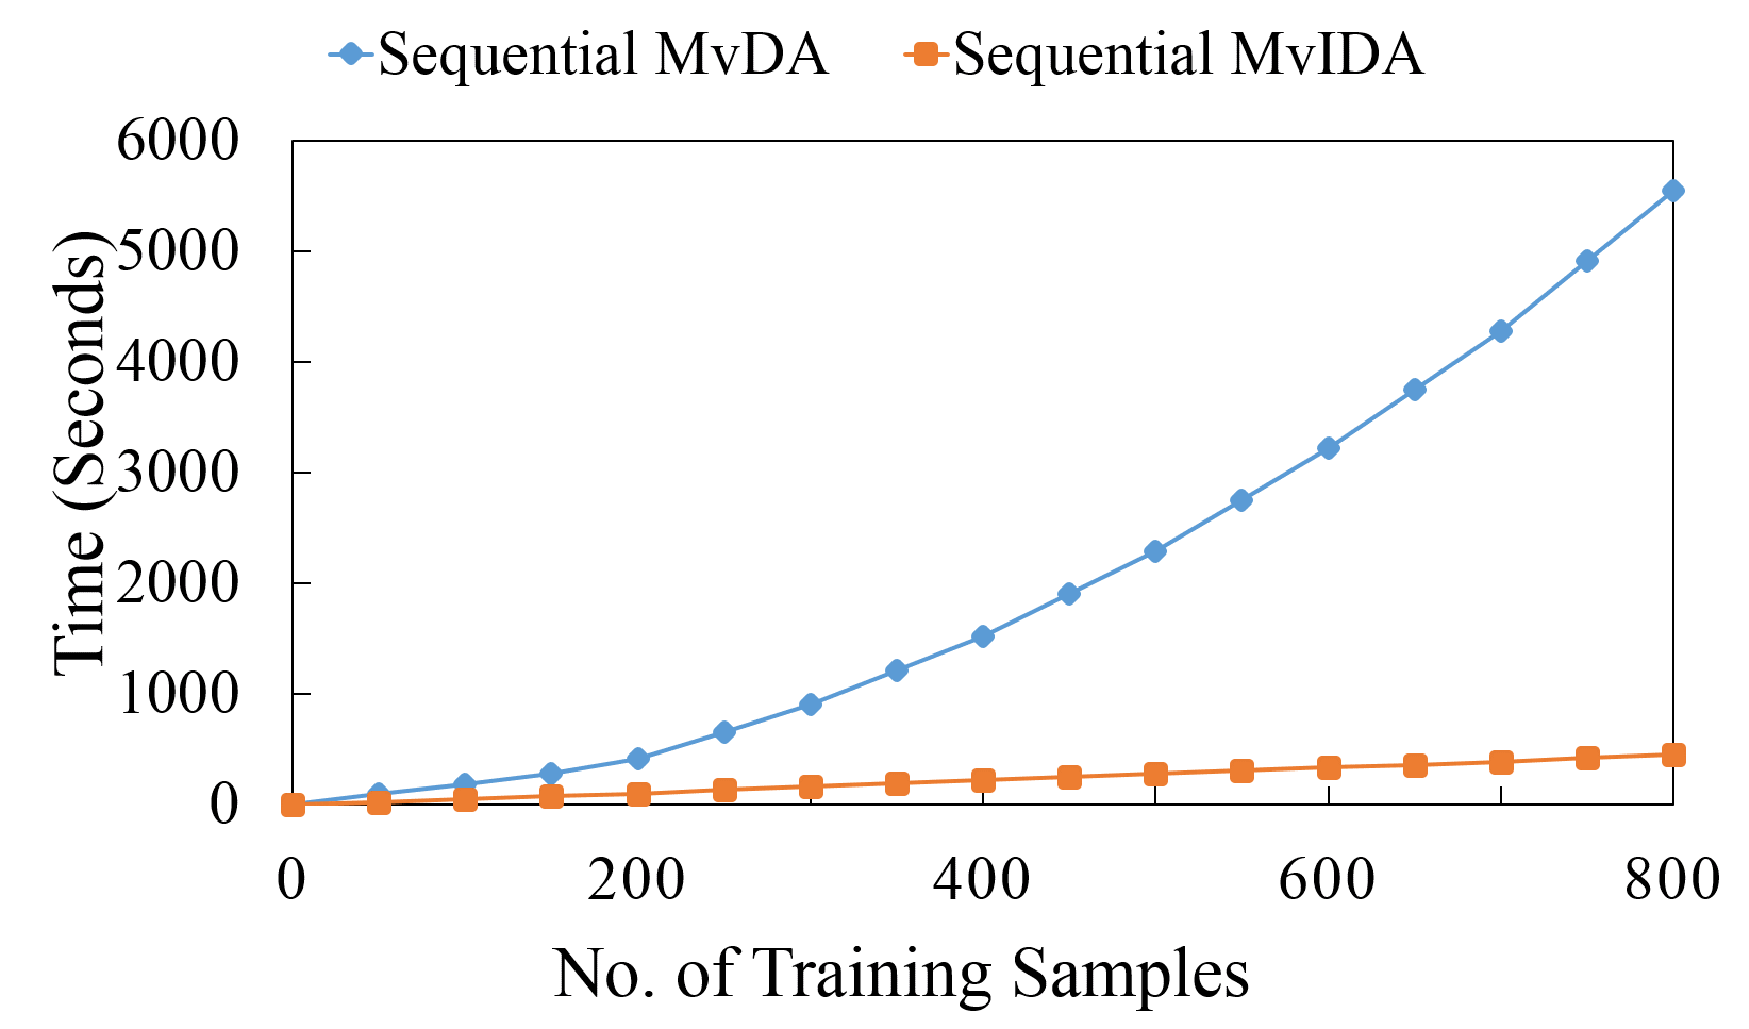
\includegraphics[width=\textwidth]{Figures/MvIDA/Fig9.pdf}
    \caption{{\scriptsize Caltech-7 Dataset}}
    \label{fig:MvIDA_Time_Seq_Cal}
  \end{subfigure}

  \begin{subfigure}[h]{0.40\textwidth}
    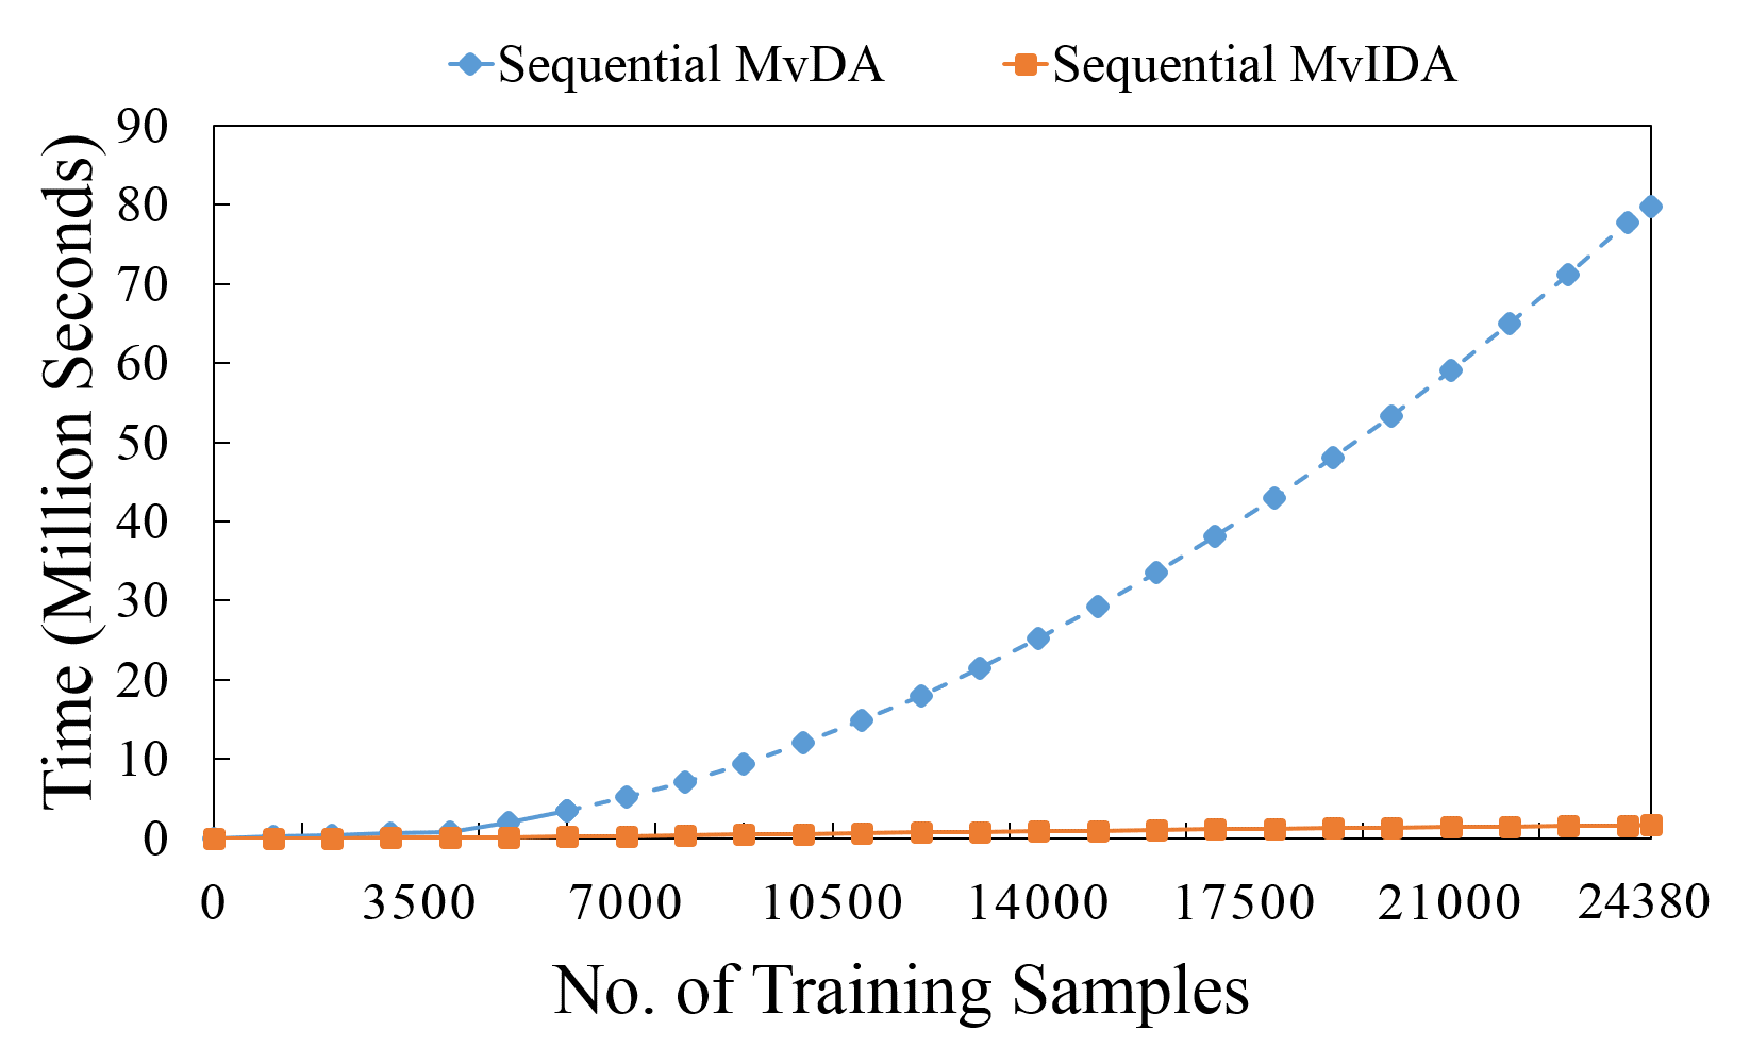
\includegraphics[width=\textwidth]{Figures/MvIDA/Fig10.pdf}
    \caption{{\scriptsize AwA Dataset}}
    \label{fig:MvIDA_Time_Seq_AwA}
  \end{subfigure}
\caption{Comparison of training time of MvIDA and batch MvDA : sequential increment}
\label{fig:MvIDA_Time_Seq}
\end{figure*}

\begin{figure*}[t]
\centering
  \begin{subfigure}[h]{0.40\textwidth}
    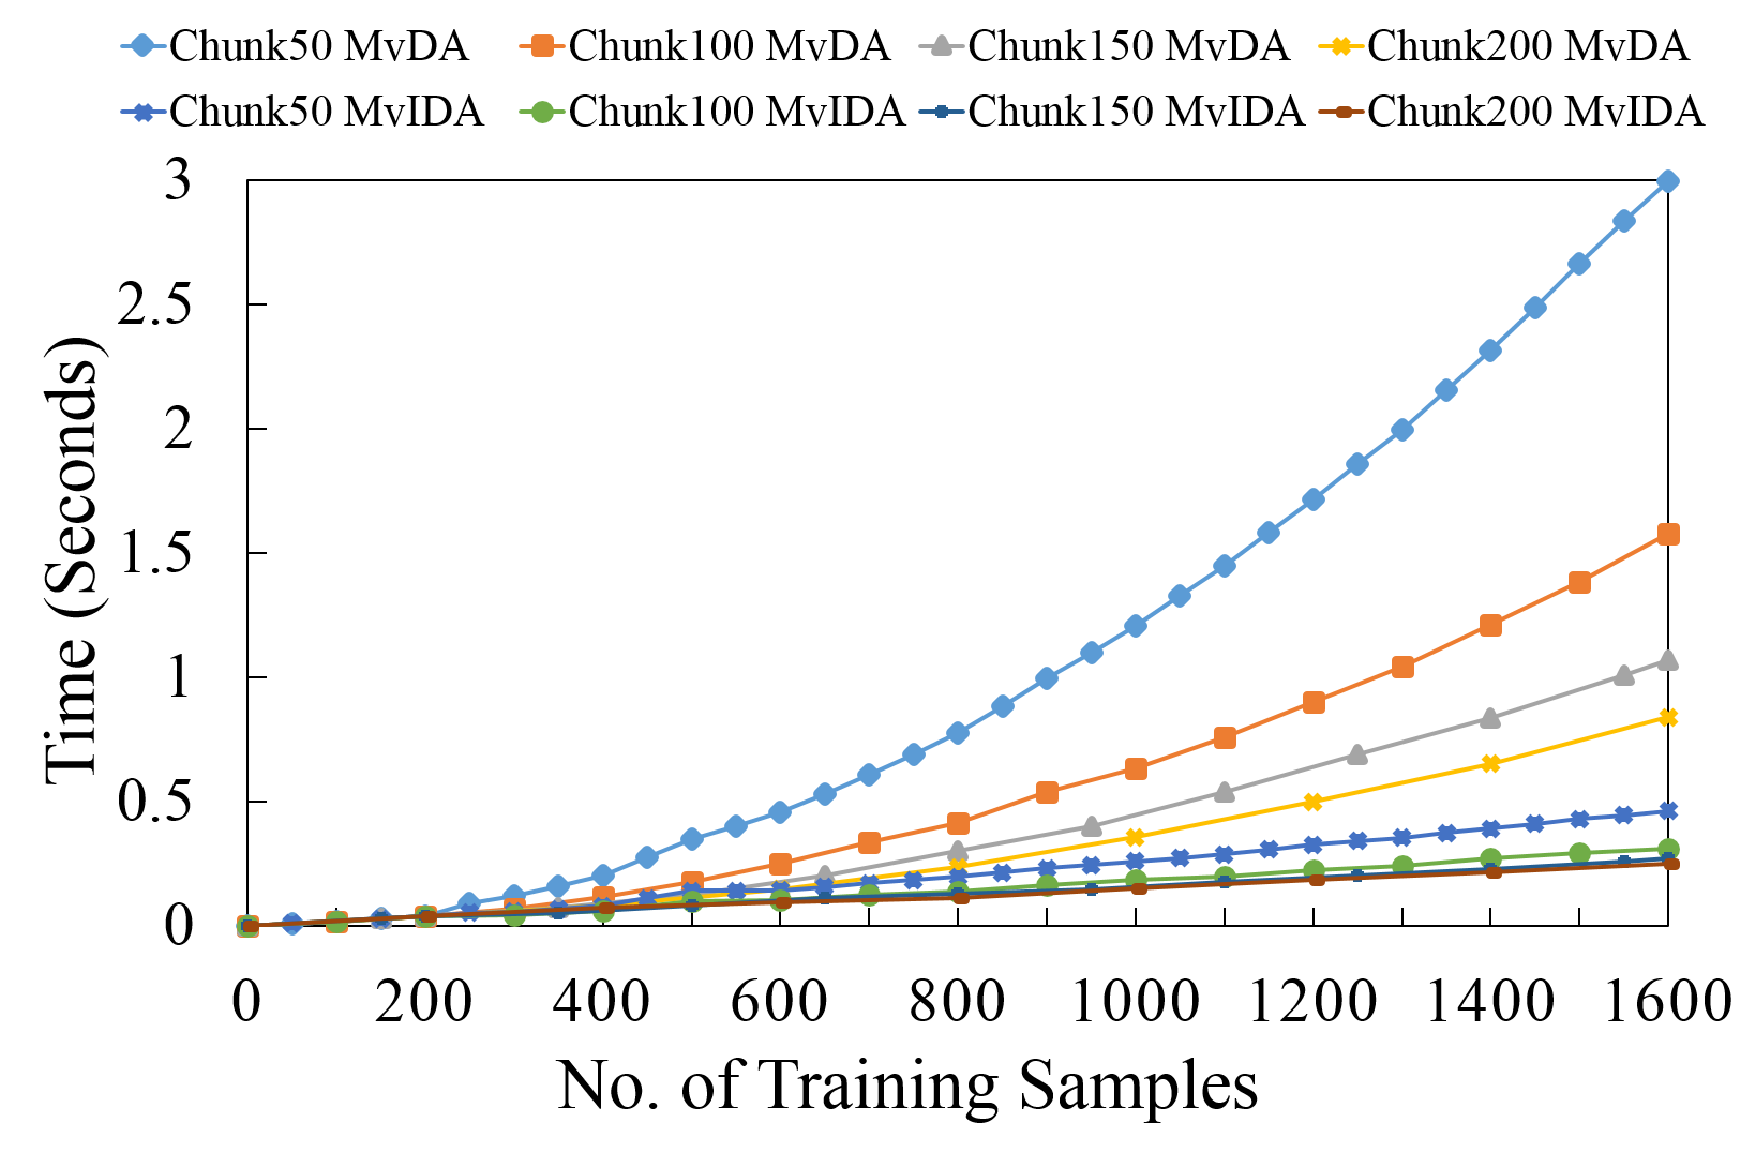
\includegraphics[width=\textwidth]{Figures/MvIDA/Fig11.pdf}
    \caption{{\scriptsize Handwritten Digits Dataset}}
    \label{fig:MvIDA_Time_Chk_Dig}
  \end{subfigure}
  \begin{subfigure}[h]{0.40\textwidth}
    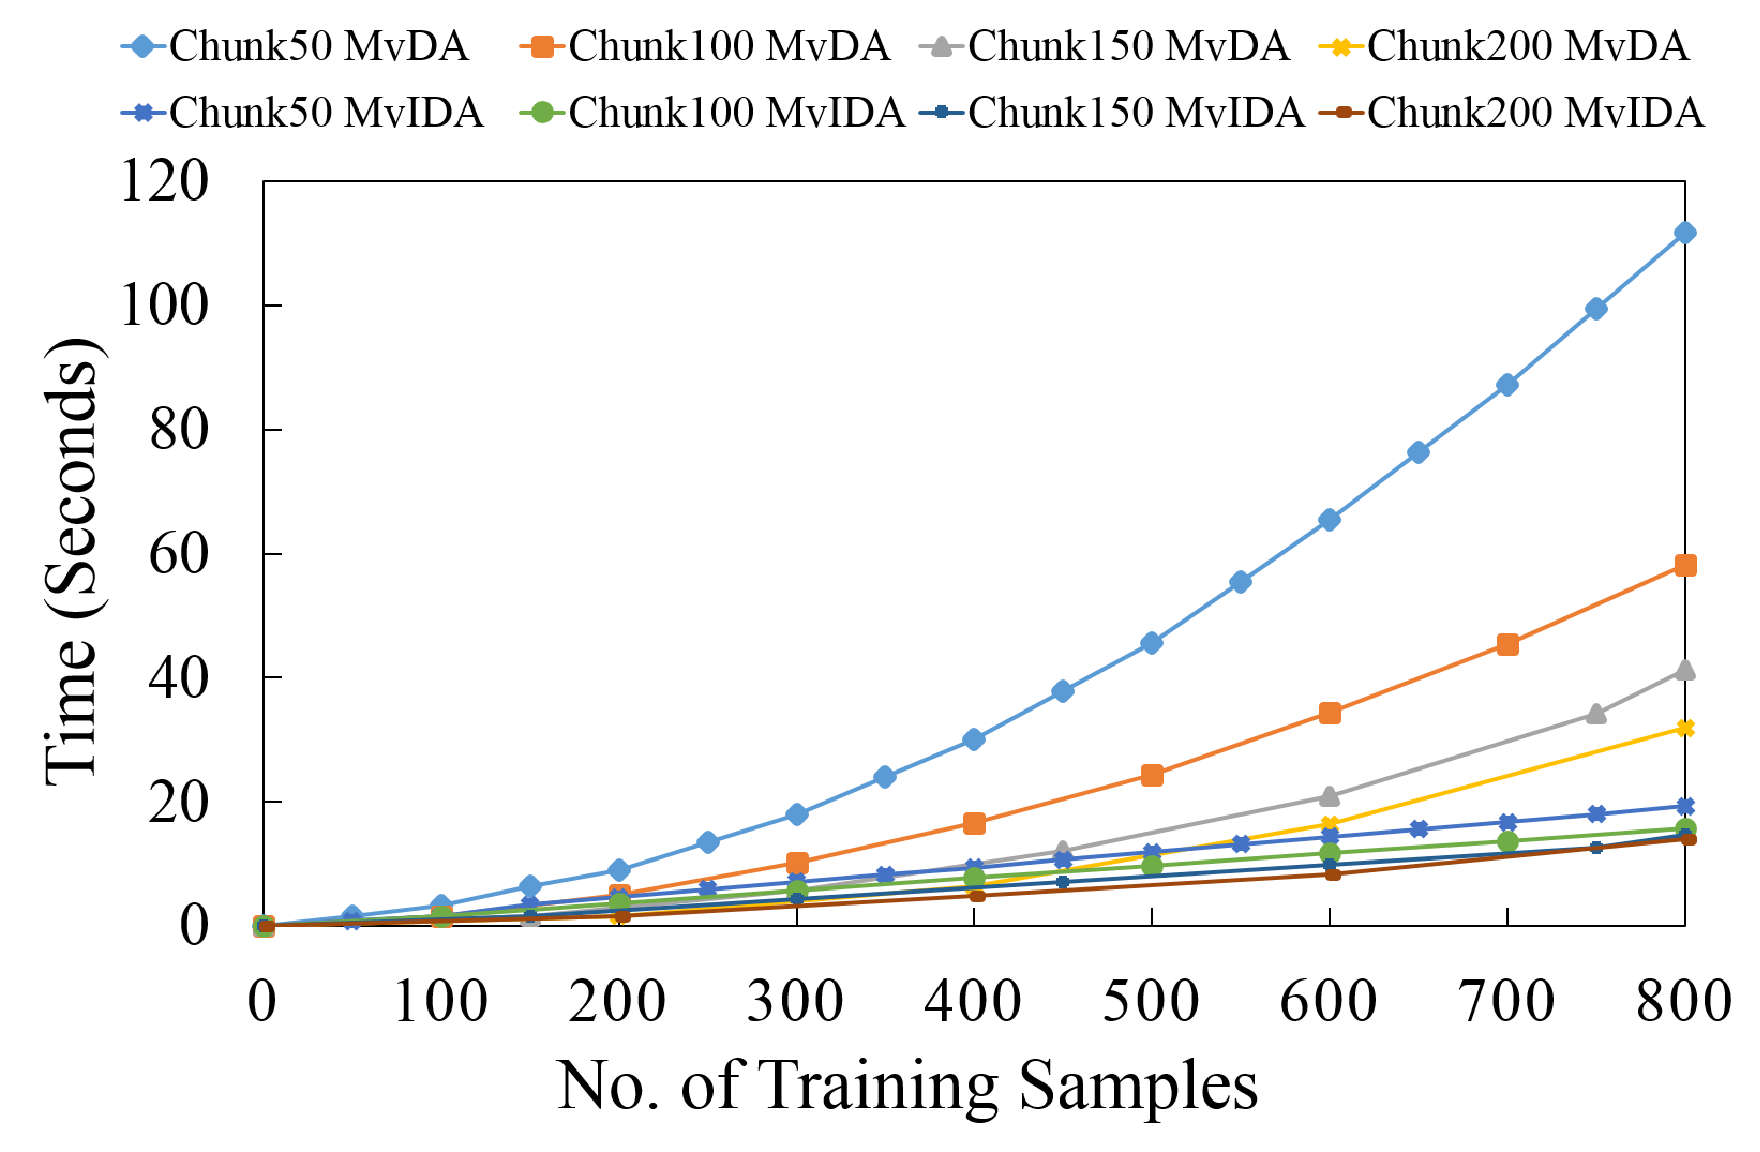
\includegraphics[width=\textwidth]{Figures/MvIDA/Fig12.pdf}
    \caption{{\scriptsize Caltech-7 Dataset}}
    \label{fig:MvIDA_Time_Chk_Cal}
  \end{subfigure}
  
  \begin{subfigure}[h]{0.40\textwidth}
    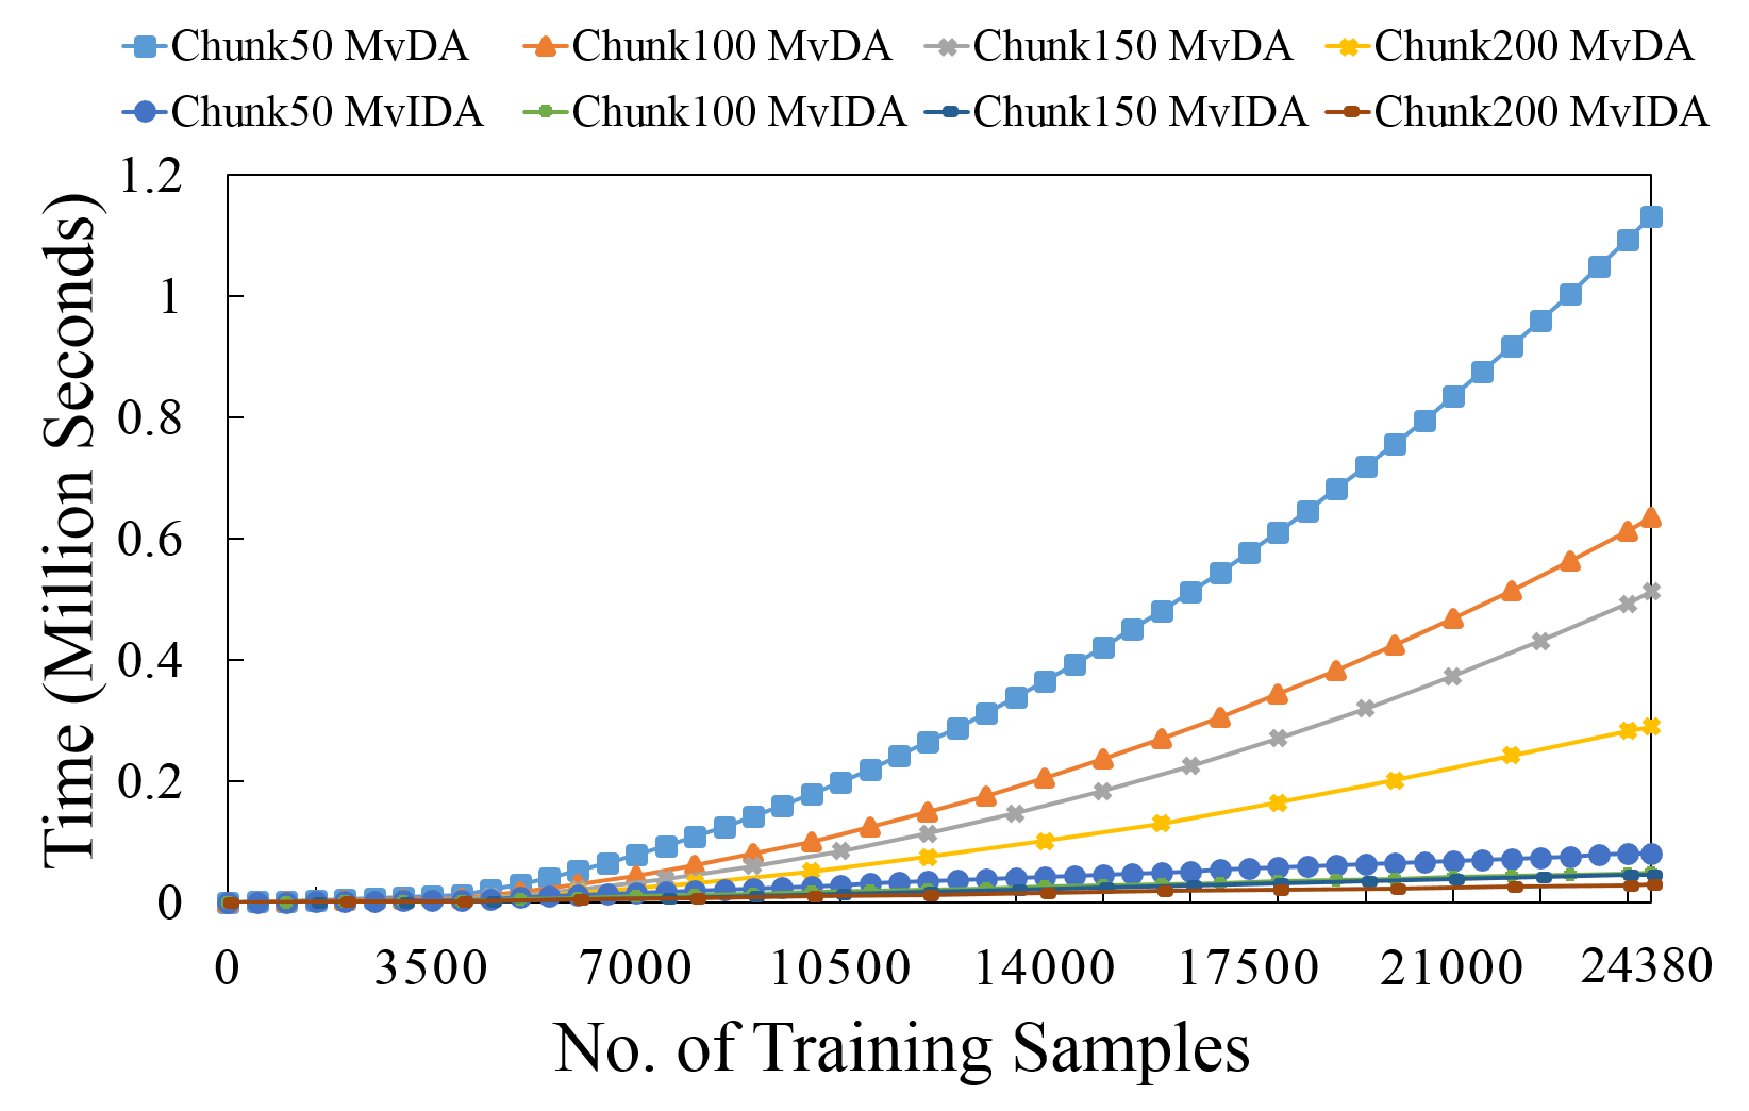
\includegraphics[width=\textwidth]{Figures/MvIDA/Fig13.pdf}
    \caption{{\scriptsize AwA Dataset}}
    \label{fig:MvIDA_Time_Chk_AwA}
  \end{subfigure}
\caption{Comparison of training time of MvIDA and batch MvDA : chunk increment}
\label{fig:MvIDA_Time_Chk}
\end{figure*}
\clearpage


%\noindent

Fig.\ref{fig:MvIDA_Time_Chk} shows the time comparison between MvIDA and batch MvDA for chunk increment. It shows training time for each of the four chunk sizes (50, 100, 150, and 200) for both methods. The time course of MvIDA is represented by four lines at the bottom of the graph that arecloser to each other. In this case also, we observe that the time required by batch MvDA sees a faster growth and is much higher than that of the MvIDA.
\end{itemize}








\subsubsection{Memory Usage}
\label{ssubs:MvIDA_Memory}
\begin{itemize}
\item \textbf{RQ4 :} 
Can this incremental method reduce memory requirements?

\item \textbf{Experiment :}
We record the memory requirements of MvIDA at the intervals of 50 data points for \textit{sequential} and \textit{chunk-50}. For \textit{chunk-100}, \textit{chunk-150} and \textit{chunk-200} the time is recorded at intervals of 100, 150 and 200 data samples respectively. Memory requirements of batch MvDA are recorded by taking chunks of 100 data samples at a time.

\item \textbf{Discussion :}
The memory usage comparison between these methods for the Handwritten Digits dataset is shown in Fig. \ref{fig:MvIDA_Memory}. We see that the memory requirement of the sequential and the chunk MvIDA is less than that of the batch learning method. The sequential MvIDA requires almost constant memory as it stores only the model $\phi$ and one new data sample. Chunk MvIDA requires more space as, along with the model, it needs space for the new chunk of the data. The memory requirements of chunk increment vary according to the chunk size.

Batch MvDA, on the other hand, stores the model $\phi$ along with all the old and new data. Hence, the storage requirements are high and increase with the increments in the data.
\end{itemize}

\begin{figure}[t]
	\centering
	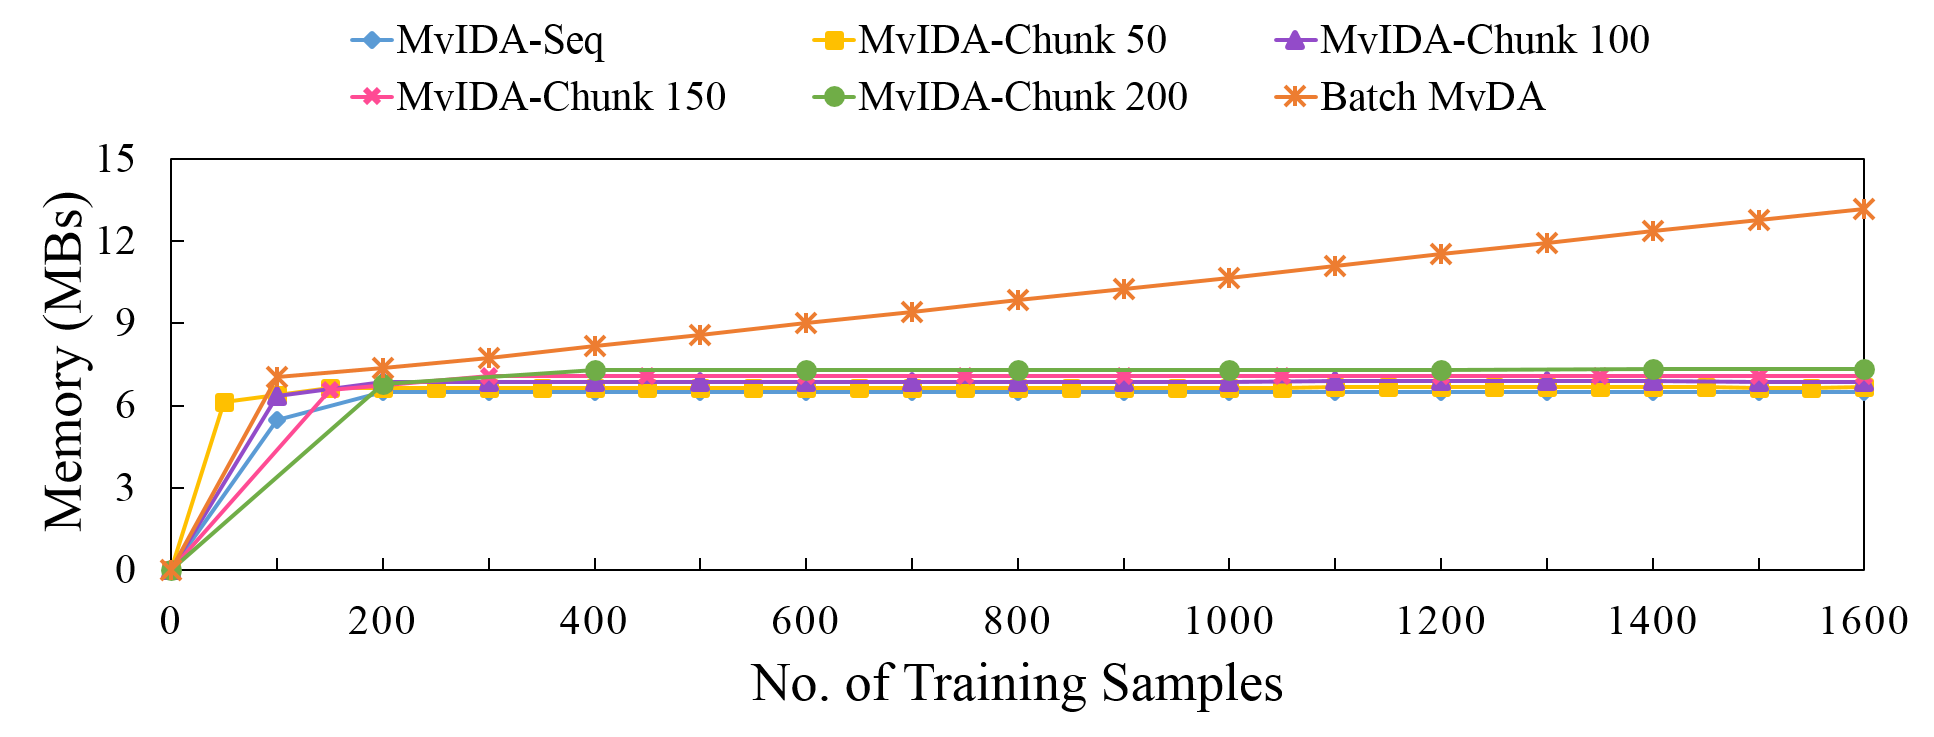
\includegraphics[width=\textwidth]{Figures/MvIDA/Fig14.png}
	\caption{Memory usage comparison for handwritten digits dataset}
	\label{fig:MvIDA_Memory}
\end{figure}








\subsubsection{Comparison with single-view ILDA}
\label{ssubs:MvIDA_ILDA}
\begin{itemize}
\item \textbf{RQ5 :} 
Is this multi-view incremental method more advantageous than a single-view incremental method in terms of classification accuracy and training time?

\item \textbf{Experiment :}
As ILDA is a single-view incremental method, to use it on multi-view data, we concatenate all the views together to form a single view and then apply ILDA on it. We record the training time and classification accuracy for sequential and chunk-100 increments using both methods.

\item \textbf{Discussion :}
The results in Table \ref{tab:MvIDA_ILDA} show the importance of using a multi-view method for multi-view data. MvIDA processes the views separately and provides far better classification results than ILDA. As all the views were concatenated together, ILDA could not use the discriminatory information provided by different views. It instead weighed all the views on the same scales, leading to misinformation and low classification accuracy. MvIDA also requires less training time than ILDA.
\end{itemize}

\begin{table}[t]
	\centering
	\caption{Comparison of accuracy and training time : MvIDA vs. single-view ILDA}
	\label{tab:MvIDA_ILDA}
	\resizebox{\columnwidth}{!}{
	\begin{tabular}{|c|c c|r r|r r|} \hline
		
		& \multicolumn{2}{c|}{} & \multicolumn{4}{c|}{\textbf{Total Training Time (Seconds)}} \\ \cline{4-7}
		\textbf{Dataset} & \multicolumn{2}{c|}{\textbf{Accuracy (\%)}} & \multicolumn{2}{c|}{\textbf{Chunk-100}} & \multicolumn{2}{c|}{\textbf{Sequential}} \\ \cline{4-7}
		& \textbf{MvIDA} & \textbf{ILDA} & \textbf{MvIDA} & \textbf{ILDA} & \textbf{MvIDA} & \textbf{ILDA} \\ \hline
		Handwritten Digits & 99.00 & 52.75 & 0.40\hspace{0.2cm} & 20.42 & 22.44\hspace{0.2cm} & 69.60 \\ 
		Caltech-7 & 97.00 & 66.50 & 19.41\hspace{0.2cm} & 564.70 & 465.72\hspace{0.2cm} & 1117.53 \\
		AwA & 96.55 & 81.62 & 49506.07\hspace{0.2cm} & 130043.42 & 1666955.69\hspace{0.2cm} & 1811942.66 \\  \hline

	\end{tabular}
	}
\end{table}















\section{Summary}
\label{sec:MvIDA_conc}
We have proposed Multi-view Incremental Discriminant Analysis (MvIDA), an incremental method for multi-view data in the dimensionality reduction paradigm. Two approaches, namely sequential MvIDA and chunk MvIDA, have been proposed to incrementally construct a common discriminant space for multi-view data.

We show that MvIDA achieves a common discriminant subspace identical to the one constructed by batch MvDA. Hence, their classification accuracy is also the same. The classification accuracy increases with the number of views. We also show that though it produces the same results, MvIDA requires much less training time and memory than batch MvDA. Also, MvIDA is invariant to the input order of the data and handles data samples from new classes at any stage of training. MvIDA also requires less training time than the single-view incremental method ILDA and produces better classification results. We see that chunk MvIDA requires less time than sequential MvIDA, whereas the latter requires less memory and converges to the optimum in the early stages of training. This work is published in \cite{ShivagundeNS21}.

The next chapter presents a batch classification method for 2D multi-view data. This method forms a basis for an incremental method in the 2D learning paradigm.

\chapterend
\cleardoublepage